\documentclass[diplomskirad]{fer}
% Dodaj opciju upload za generiranje konačne verzije koja se učitava na FERWeb
% Add the option upload to generate the final version which is uploaded to FERWeb


\usepackage{blindtext}
\usepackage[siunitx, fulldiodes, americanvoltages]{circuitikz}
\usepackage{tikz}
\usepackage{subcaption}
\usepackage{enumitem}
\usepackage{amsmath}
\usepackage[colorinlistoftodos]{todonotes}
\usetikzlibrary{shapes, calc, positioning, arrows.meta}
\usepackage{pgfplots}
% \usepackage[T1]{fontenc} % Ensures proper font encoding
% \usepackage[utf8]{inputenc} % For UTF-8 input encoding (if not already using LuaLaTeX/XeLaTeX)
\usepackage{hyperref}    % For hyperlinks and PDF features
% \usepackage{xmpincl}     % Required by pdfx for XMP metadata
% \usepackage[a-2b,mathxmp]{pdfx}[2018/12/22]
\pgfplotsset{compat=1.18}

\begin{filecontents*}[overwrite]{\jobname.xmpdata}
	\Title{Electronic speed control of a brushless DC motor for drones}
	\Author{Vlado Perković}
	\Language{hr-HR} % Set appropriate language code
	\Subject{Diplomski rad - Upravljanje brzinom vrtnje istosmjernih motora bez četkica kod bespilotnih letjelica}
	\Keywords{istosmjerni motor bez četkica\sep BLDC\sep elektroničko upravljanje brzinom\sep ESC\sep bespilotne letjelice\sep dronovi\sep komutacija u šest koraka\sep protuelektromotorna sila\sep PEMS\sep bezosjetilno upravljanje}
\end{filecontents*}
%--- PODACI O RADU / THESIS INFORMATION ----------------------------------------

% Naslov na engleskom jeziku / Title in English
\title{Electronic speed control of a brushless DC motor for drones}

% Naslov na hrvatskom jeziku / Title in Croatian
\naslov{Upravljanje brzinom vrtnje istosmjernih motora bez četkica kod bespilotnih letjelica}

% Broj rada / Thesis number
\brojrada{1150}

% Autor / Author
\author{Vlado Perković}

% Mentor 
\mentor{doc. dr. sc. Leonardo Jelenković}

% Datum rada na engleskom jeziku / Date in English
\date{September, 2025}

% Datum rada na hrvatskom jeziku / Date in Croatian
\datum{rujan, 2025.}

%-------------------------------------------------------------------------------

% tikz postavke
\tikzset{dot/.style={fill,circle,minimum size=4pt,inner sep=0pt}}

\begin{document}

% Naslovnica se automatski generira / Titlepage is automatically generated
\maketitle

%--- ZADATAK / THESIS ASSIGNMENT -----------------------------------------------

% Zadatak se ubacuje iz vanjske datoteke / Thesis assignment is included from external file
% Upiši ime PDF datoteke preuzete s FERWeb-a / Enter the filename of the PDF downloaded from FERWeb
\zadatak{hr_0036535500_90.pdf}

%--- ZAHVALE / ACKNOWLEDGMENT --------------------------------------------------

\begin{zahvale}
	% Ovdje upišite zahvale / Write in the acknowledgment
	Hvala na čaju...
\end{zahvale}

% Odovud započinje numeriranje stranica / Page numbering starts from here
\mainmatter

% Sadržaj se automatski generira / Table of contents is automatically generated
\tableofcontents
\listoftodos{}
\newpage

%--- UVOD / INTRODUCTION -------------------------------------------------------
\chapter{Uvod}
\label{pog:uvod}

% --- KRATKI UVOD U TEMATIKU ---
Bespilotne letjelice (eng. \textit{Unmanned Aerial Vehicle, UAV}), popularno
zvane dronovi, danas se široko primjenjuju u brojnim industrijama, od filmske
produkcije i poljoprivrede do dostave i rekreacijskog letenja
\cite{cite:primjena}. Iako postoje različite konstrukcije, poput bespilotnih
letjelica s fiksnim krilima, višerotorske bespilotne letjelice prevladavaju u
modernim primjenama. Osnovu njihovog pogona čini istosmjerni motor bez četkica
(eng. \textit{Brushless DC motor, BLDC}), čije karakteristike poput visoke
učinkovitosti, pouzdanosti i dobrog omjera snage i mase omogućuju razvoj
agilnih i energetski učinkovitih letjelica. Performanse drona, uključujući
stabilnost, vrijeme leta i agilnost, izravno ovise o sposobnosti preciznog i
brzog upravljanja brzinom vrtnje ovih motora \cite{cite:karakteristike_motora}.

% --- UPRAVLJANJE BRZINOM VRTNJE ---

Upravljanje brzinom vrtnje motora BLDC postiže se održavanjem kuta između polja
rotora i statora. Za to upravljač mora znati položaj rotora što se obično
postiže osjetilima Hallovog učinka ili enkoderima pozicije. Postoje i metode
upravljanja koje ne koriste osjetila za određivanje položaja rotora. One
smanjuju troškove, složenost i masu sustava što ih čini pogodnijim izborom za
dronove. Kod metode komutacije u šest koraka popularna je tehnika praćenja
protuelektromotorne sile (PEMS) u kojoj upravljač zaključuje položaj rotora
praćenjem PEMS-a koji se inducira u nevođenoj fazi (odjeljak
\ref{sec:six-step}). Složenije metode komutacije poput sinusne komutacije i
vektorskog upravljanja koriste algoritme za estimaciju položaja rotora jer
nemaju mogućnost mjerenja PEMS-a \cite{NXP_AN2355}.

% --- OPIS RADA I CILJA ---
\todo[inline]{nadopuni opis rada}
Ovaj rad bavi se analizom, modeliranjem, simulacijom i implementacijom sustava
za upravljanje brzinom vrtnje motora BLDC s naglaskom na primjenu kod
bespilotnih letjelica. Cilj je istražiti i implementirati sustav upravljanja
bez korištenja osjetila temeljen na metodi komutacije u šest koraka. Kroz
rad će se analizirati i temeljni kompromisi u dizajnu motora, poput izbora
konfiguracije namotaja, kako bi se razumio njihov utjecaj na konačne
performance.

\todo[inline]{popravi pregled poglavlja}
Drugo poglavlje daje teorijsku podlogu o motorima BLDC. Treće poglavlje
detaljno opisuje upravljanje motora BLDC bez osjetila, s fokusom na komutaciju
u šest koraka. Četvrto poglavlje prikazuje sklopovlje sustava, opisuje odabrani
elektronički sklop za upravljanje brzinom (eng. \textit{Electronic Speed
	Controller, ESC}) te odabrani motor. Peto poglavlje opisuje implementaciju
razvijenog algoritma na odabranom sklopovlju, dok šesto poglavlje donosi zaključak i sažima rezultate rada.
%-------------------------------------------------------------------------------
\chapter{Istosmjerni elektromotor bez četkica}
\label{pog:bldc}
\section{Osnove i konstrukcija}
\label{sec:bldc:uvod}

Istosmjerni elektromotor bez četkica, poznat i kao beskolektorski istosmjerni
motor ili elektronički komutirani motor, vrsta je elektromotora sa stalnim
magnetima čija je temeljna značajka rad bez mehaničkog kolektora i četkica.

Konstrukcija motora BLDC sastoji se od stacionarnog dijela, statora, i
rotirajućeg dijela, rotora. U statoru su smještene zavojnice, bakreni namotaji
koji djeluju kao elektromagneti. Na rotoru su stalni magneti
\cite{elektromotor-beskolektorski}. Postoji unutarnji ili \textit{ inrunner }
motor kod kojeg se rotor nalazi unutar statora. Unutarnji motori općenito imaju
manji moment tromosti i sposobni su za veće brzine vrtnje \cite{cite:bldc}.
Isto tako postoji i vanjski ili \textit{ outrunner } motor kojem je rotor
izvana i okružuje stator. Ovakvi motori obično daju veći okretni moment pri
nižim brzinama vrtnje \cite{cite:bldc}.

\missingfigure{umetni sliku presjeka motora}

Valja spomenuti kako uz motore BLDC usko se vežu sinkroni elektromotori sa
stalnim magnetima (\textit{Permanent Magnet Synchronous Motor, PMSM}). Takvi
motori također su vrsta elektromotora sa stalnim magnetima i glavna je razlika
valni oblik protuelektromotorne sile gdje motor BLDC ima trapezni oblik, a
motor PMSM ima sinusni oblik. Dalje u radu oslanjat će se na motore BLDC iako
većina stvari vrijedi i za motore PMSM
\cite{elektromotor-sa-stalnim-magnetima}.

Rad motora bez četkica temelji se na kontroliranoj interakciji između
magnetskog polja rotora, kojeg čine permanentni magneti, i rotirajućeg
magnetskog polja statora. Za razliku od klasičnih istosmjernih motora,
rotirajuće polje statora ovdje se stvara elektronički, bez mehaničkog kolektora
i četkica. Taj zadatak obavlja upravljački sklop ESC, koji sekvencijalnim
napajanjem statorskih namota precizno sinkronizira polje statora s položajem
rotora \cite{cite:disertacija}. Cilj je održavati optimalan kut između njihovih
magnetskih vektora kako bi se maksimizirao okretni moment. Zbog dobrog
kompromisa između performansi i složenosti izvedbe, u praksi se najčešće
koriste trofazni motori \cite{cite:trofazni}, čiji su namoti prostorno
razmaknuti za 120 električnih stupnjeva \cite{MicrochipAN885}.

Potpunim uklanjanjem kolektora i četkica izbjegavaju se najveći nedostaci
klasičnih istosmjernih strojeva kao što su, osim već navedenog mehaničkog
trošenja i čestog održavanja, iskrenje, i ograničen vijek trajanja. Zbog svoje
pouzdanosti, učinkovitosti često i preko 80\% \cite{motor-ucinkovitost} i
mogućnosti postizanja iznimno velikih brzina (preko 70 000 okretaja u minuti
\cite{motor-rpm}), beskolektorski se motori danas široko primjenjuju u
sustavima kao što su bespilotne letjelice, servopogoni, pogoni tvrdih diskova u
računalima, medicinski uređaji, moderni alatni strojevi te u audio i video
tehnici.

\newpage

\section{Matematički model motora}
\label{sec:mat_model}
Za trofazne motore, električni odnosi mogu se modelirati sljedećim nizom jednadžbi izvedenih iz reference \cite{}. Jednadžbe prate sliku \ref{fig:wye-math}.
\begin{align}
	V_{an} & = R \cdot i_a + \frac{d}{dt}(L_{aa}i_a + L_{ab}i_b + L_{ac}i_c) + V_{ea} \\
	V_{bn} & = R \cdot i_b + \frac{d}{dt}(L_{ba}i_a + L_{bb}i_b + L_{bc}i_c) + V_{eb} \\
	V_{cn} & = R \cdot i_c + \frac{d}{dt}(L_{ca}i_a + L_{cb}i_b + L_{cc}i_c) + V_{ec}
\end{align}
pri čemu su:
\begin{itemize}
	\item $V_{an}, V_{bn}, V_{cn}$ -- fazni naponi u odnosu na neutralnu točku motora $n$,
	\item $i_a, i_b, i_c$ -- fazne struje,
	\item $V_{ea}, V_{eb}, V_{ec}$ -- protuelektromotorne sile,
	\item $R$ -- otpori statorskog namota po fazi, koji su jednaki za sve tri faze,
	\item $L_{aa}, L_{bb}, L_{cc}$ -- vlastiti induktiviteti,
	\item $L_{ab}, L_{ba}, L_{ac}, L_{ca}, L_{bc}, L_{cb}$ -- međusobni induktiviteti.
\end{itemize}
Ako se pretpostavi da su faze simetrične i da magnetska reluktancija ne ovisi o
električnom kutu rotora, tada su tri vlastita induktiviteta jednaka, a šest
međusobnih induktiviteta također je međusobno jednako:
\begin{equation}
	L_{aa} = L_{bb} = L_{cc} = L_v \tag{2.4}
\end{equation}
\begin{equation}
	L_{ab} = L_{ba} = L_{ac} = L_{ca} = L_{bc} = L_{cb} = M \tag{2.5}
\end{equation}
Ekvivalentni induktivitet $L$ može se izračunati kao:
\begin{equation}
	L = L_v - M \tag{2.6}
\end{equation}
Uz pretpostavku simetričnih faznih struja, vrijedi:
\begin{equation}
	i_a + i_b + i_c = 0 \tag{2.7}
\end{equation}
Tada se električni odnosi mogu pojednostavniti, a motor BLDC modelirati na
sljedeći način:
\begin{align}
	V_{an} & = R \cdot i_a + L\frac{di_a}{dt} + V_{ea} \\
	V_{bn} & = R \cdot i_b + L\frac{di_b}{dt} + V_{eb} \\
	V_{cn} & = R \cdot i_c + L\frac{di_c}{dt} + V_{ec}
\end{align}
\begin{figure}[h!]
	\centering
	\begin{circuitikz}[european, cute inductors]
		\path (0,0) coordinate(n) node[above,red]{$n$};
		\draw(n)
		to[short] ++(-90:0.4)
		to[V , V>=$V_{ec}$] ++(-90:1.2)
		to[L , L=$L_c$] ++(-90:1.2)
		to[R , R=$R_c$] ++(-90:1.2)
		to[short] ++(-90:0.4)
		coordinate(c) node[left,red]{$c$};
		\draw(n)
		to[short] ++(30:0.4)
		to[V , V>=$V_{eb}$] ++(30:1.2)
		to[L , L=$L_b$] ++(30:1.2)
		to[R , R=$R_b$] ++(30:1.2)
		to[short] ++(30:0.4)
		coordinate(b) node[above,red]{$b$};
		\draw(n)
		to[short] ++(150:0.4)
		to[V , V>=$V_{ea}$] ++(150:1.2)
		to[L , L=$L_a$] ++(150:1.2)
		to[R , R=$R_a$] ++(150:1.2)
		to[short] ++(150:0.4)
		coordinate(a) node[left,red]{$a$};
		\draw (a) node[dot] {};
		\draw (b) node[dot] {};
		\draw (c) node[dot] {};
		\draw (n) node[dot] {};
	\end{circuitikz}
	\caption{Električna shema motora}
	\label{fig:wye-math}
\end{figure}
\newpage

\section{Protuelektromotorna sila}
Protuelektromotorna sila (eng. \textit {Counter-electromotive force,
	Back-electromotive force, back-EMF}) je napon koji se stvara u zavojnicama
statora prilikom vrtnje rotora, a suprotstavlja se naponu napajanja. Ovaj se
napon inducira u skladu s Faradayevim zakonom elektromagnetske indukcije.

Oblik protuelektromotorne sile ovisi o mehaničkoj konstrukciji motora,
ponajviše o raspodjeli i obliku permanentnih magneta na rotoru te o izvedbi
statorskih namota. Ovisno o tome, postoje trapezoidalni valni oblik (slika
\ref{fig:trapezoid}) i sinusoidalni valni oblik (slika \ref{fig:sine})
protuelektromotorne sile.

Poznavanje valnog oblika protuelektromotorne sile postaje važno pri upravljanju
okretanja elektromotora jer se valni oblici pokretačkog signala i PEMS-a moraju
poklapati za minimizaciju valovitosti momenta (odjeljak
\ref{trap:torque-ripple}) \cite{MicrochipAN885}.

\begin{figure}[h!]
	\centering
	\captionsetup[subfigure]{skip=10pt}
	\begin{subfigure}[b]{0.48\textwidth}
		\centering
		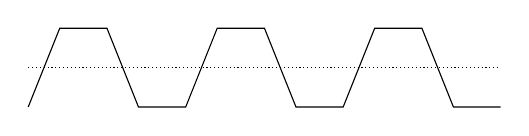
\begin{tikzpicture}[yscale=0.5]
			\begin{scope}[local bounding box=trapezoid]
				\draw [densely dotted] (0,0)  -- +(6,0);
				\draw (0,-1) foreach \x in {1,2,3} { -- ++(0.4,2) -- ++(0.6,0) -- ++(0.4,-2) -- ++(0.6,0) };
			\end{scope}
		\end{tikzpicture}
		\subcaption{Trapezoidalni valni oblik}
		\label{fig:trapezoid}
	\end{subfigure}
	\hfill
	\begin{subfigure}[b]{0.48\textwidth}
		\centering
		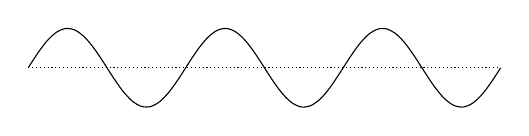
\begin{tikzpicture}[yscale=0.5]
			\begin{scope}[local bounding box=sine]
				\draw [densely dotted] (0,0)  -- +(6,0);
				\draw plot[domain=0:6,variable=\x,samples=51,smooth] (\x,{sin(deg(\x*pi))});
			\end{scope}
		\end{tikzpicture}
		\subcaption{Sinusoidalni valni oblik}
		\label{fig:sine}
	\end{subfigure}

	\caption{Usporedba valnih oblika PEMS-a}
	\label{fig:waveforms}
\end{figure}

\newpage

\section{Konfiguracija namotaja na statoru}
\label{sec:konfiguracija_namotaja}
Na trofaznom motoru BLDC namotaji na statoru mogu biti u dvije glavne
konfiguracije:

U \textbf{zvjezdastom spoju (eng. \textit{wye, star connection})} tri zavojnice
spojene su u zajedničkoj središnjoj točki, zvjezdištu (točka \textit{n} na
slici \ref{fig:wye}). Fazni napon, $V_{\text{faza}}$ [V], niži je od mrežnog
napona, $V_{\text{mreža}}$ [V], prema izrazu $V_{\text{faza}} =
	V_{\text{mreža}} / \sqrt{3}$, a fazna struja, $I_{\text{faza}}$ [A], jednaka je
mrežnoj struji.

U \textbf{trokutnom spoju (eng. \textit{Delta connection})} zavojnice su
spojene međusobno u trokut (slika \ref{fig:delta}). Fazni napon,
$V_{\text{faza}}$ [V], jednak je mrežnom naponu, $V_{\text{mreža}}$ [V], a
fazna struja, $I_{\text{faza}}$ [A], niža je od mrežne struje,
$I_{\text{mreža}}$ [A], prema izrazu $I_{\text{faza}} = I_{\text{mreža}} /
	\sqrt{3}$.

Zbog ove razlike u faznim naponima, za dva motora s ovim konfiguracijama i
pripadnim konstantama motora $K_{t, Z}$ i $K_{t, T}$ za proizvesti jednak
moment vrijedi:

Moment, $\tau$ [Nm], može se izraziti preko izraza $\tau = K_t \cdot
	I_{\text{faza}}$, gdje je $K_t$ konstanta momenta [Nm/A], a $I_{\text{faza}}$
fazna struja [A]. Odnos konstanti momenta je $K_{t, T} = K_{t, Z} / \sqrt{3}$
\cite{cite:disertacija}.

Da bi se proizveo jednak moment, odnos faznih struja mora biti:

\begin{align*}
	K_{t,Z} \cdot I_{\text{faza},Z}  & = K_{t,T} \cdot I_{\text{faza},T}                                 \\
	K_{t,Z} \cdot I_{\text{faza},Z}  & = \left( \frac{K_{t,Z}}{\sqrt{3}} \right) \cdot I_{\text{faza},T} \\
	\sqrt{3} \cdot I_{\text{faza},Z} & = I_{\text{faza},T}
\end{align*}
Ovaj rezultat pokazuje da za isti moment, fazna struja u trokutnom spoju mora biti $\sqrt{3}$ puta veća od fazne struje u zvjezdastom spoju.
Koristeći ovaj odnos, sada se mogu usporediti linijske struje ($I_L$) koje motori vuku iz izvora napajanja.
\begin{align*}
	I_{L,T} & = \sqrt{3} \cdot I_{\text{faza},T}                  &  & \text{(Definicija linijske struje za trokut)}              \\
	        & = \sqrt{3} \cdot (\sqrt{3} \cdot I_{\text{faza},Z}) &  & \text{(Uvrštavanje odnosa faznih struja)}                  \\
	        & = 3 \cdot I_{\text{faza},Z}                                                                                         \\
	        & = 3 \cdot I_{L,Z}                                   &  & \text{(Budući da je } I_{\text{faza},Z} = I_{L,Z} \text{)}
\end{align*}

Izvod pokazuje da za proizvodnju istog momenta, motor spojen u trokut zahtijeva
tri puta veću linijsku struju od motora spojenog u zvijezdu. Ova temeljna
razlika u potrebnoj struji definira njihovu primjenu koja je opisana u
sljedećem odjeljku \ref{sec:moment_brzina}.
\begin{figure}[h!]
	\centering
	\begin{subfigure}[b]{0.48\textwidth}
		\centering
		\begin{circuitikz}[american, cute inductors]
			\path (0,0) coordinate(n) node[above,red]{$n$};
			\draw(n) to[L , L=$L$, *-o] ++(-90:3) coordinate(c) node[left,red]{$c$};
			\draw(n) to[L , L=$L$, *-o] ++(30:3)  coordinate(b) node[above,red]{$b$};
			\draw(n) to[L , L=$L$, *-o] ++(150:3) coordinate(a) node[left,red]{$a$};
			\draw (a) node[dot] {};
			\draw (b) node[dot] {};
			\draw (c) node[dot] {};
			\draw (n) node[dot] {};
		\end{circuitikz}
		\caption{Zvijezda}
		\label{fig:wye}
	\end{subfigure}
	\hfill
	\begin{subfigure}[b]{0.48\textwidth}
		\centering
		\begin{circuitikz}[american, cute inductors]

			\begin{scope}[yshift=-7cm]
				\path (0,0) coordinate(n) ;
				\draw (n) ++( -30:2) coordinate(a) node[below,red]{$a$};
				\draw (n) ++(  90:2) coordinate(c) node[above,red]{$c$};
				\draw (n) ++(-150:2) coordinate(b) node[left,red]{$b$};
				\draw (c) to[L , L=$L$, o-o] (a);
				\draw (a) to[L , L=$L$, o-o] (b);
				\draw (b) to[L , L=$L$, o-o] (c);
				\draw (a) node[dot] {};
				\draw (b) node[dot] {};
				\draw (c) node[dot] {};
			\end{scope}
		\end{circuitikz}
		\caption{Trokut}
		\label{fig:delta}
	\end{subfigure}
	\caption{Konfiguracije namotaja}
	\label{fig:wye-delta}
\end{figure}

\newpage
\section{Odnos momenta i brzine vrtnje}
\label{sec:moment_brzina}

Performanse motora BLDC temelje se na kompromisu između okretnog momenta i
brzine vrtnje.

S jedne strane, okretni moment ($\tau$) izravno je proporcionalan struji ($I$)
prema izrazu $\tau = K_t \cdot I$ (odjeljak \ref{sec:konfiguracija_namotaja}).
S druge strane, rotacijom se inducira PEMS ($V_{\text{pems}}$) koji se
suprotstavlja naponu napajanja i proporcionalan je kutnoj brzini ($\omega$)
prema izrazu $V_{\text{pems}} = K_e \cdot \omega$. Porast brzine uzrokuje
porast $V_{\text{pems}}$, što smanjuje efektivni napon na namotajima, a time i
struju i raspoloživi moment. Motor dostiže svoju maksimalnu brzinu, odnosno
brzinu praznog hoda, kada se $V_{\text{pems}}$ približi naponu napajanja, čime
se moment smanjuje na nulu (zanemarujući trenje) što se može vidjeti na slici
\ref{fig:torque_speed}. U zoni kontinuiranog momenta porast brzine ne utječe na
moment i to područje je omeđeno nazivnim momentom i nazivnom brzinom.

\begin{figure}[h!]
	\centering
	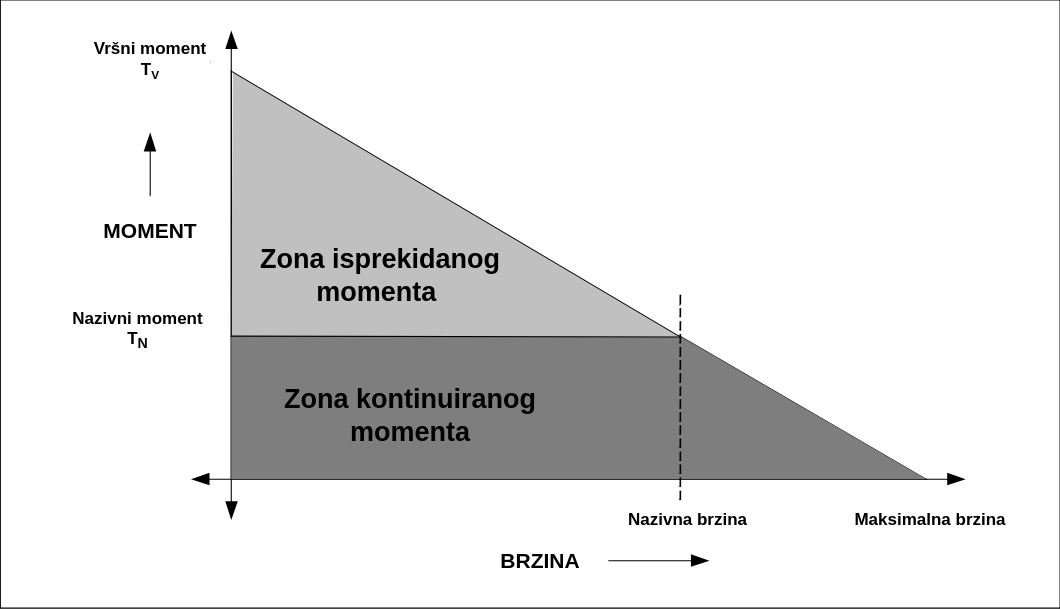
\includegraphics[width=\textwidth]{Figures/microchip_torque_speed.png}
	\caption{Graf omjera momenta i brzine (prilagođeno prema \cite{MicrochipAN885})}
	\label{fig:torque_speed}
\end{figure}

Na ovaj kompromis presudno utječe konfiguracija namotaja statora, kao što je
opisano u odjeljku \ref{sec:konfiguracija_namotaja}. Budući da su konstante
$K_t$ i $K_e$ povezane, izbor konfiguracije definira momentnu karakteristiku
motora.

\begin{itemize}
	\item \textbf{Zvjezdasti spoj -} Zbog veće efektivne duljine namotaja, ova konfiguracija ima višu konstantu momenta ($K_t$) i posljedično višu konstantu protuelektromotorne sile ($K_e$). To rezultira visokom momentnom učinkovitošću (veći moment po amperu), ali i nižom maksimalnom brzinom jer $V_{\text{pems}}$ brže doseže napon napajanja.

	\item \textbf{Trokutni spoj -} Ova konfiguracija ima niži $K_t$ i $K_e$ (za faktor $\sqrt{3}$). Kao što je spomenuto u odjeljku \ref{sec:konfiguracija_namotaja}, za isti moment zahtijeva znatno veću struju, što smanjuje učinkovitost. Međutim, niži $K_e$ omogućuje motoru postizanje veće maksimalne brzine prije nego što $V_{\text{pems}}$ postane ograničavajući faktor.
\end{itemize}

Izbor između ove dvije konfiguracije stoga predstavlja inženjerski kompromis.
Zvjezdasti spoj preferira se u primjenama gdje su prioritet visoki moment pri
nižim brzinama i energetska učinkovitost, poput dronova za snimanje. S druge
strane, trokutni spoj odabire se za primjene gdje je cilj postizanje maksimalne
brzine, kao kod trkaćih dronova FPV, čak i po cijenu veće potrošnje struje.

\newpage

\chapter{Upravljanje motorom BLDC bez osjetila položaja}
\label{pog:bldc_upravljanje_bez_senzora}

Metoda koja se koristi za upravljanje motorom BLDC utječe na izvedbu motora,
njegovu učinkovitost i glatkoću rada. Odabir metode upravljanja ovisi o
karakteristikama motora kao što je valni oblik PEMS-a i zahtjevima primjene
\cite{cite:bldc}. Ovaj rad koristi metodu komutacije u šest koraka s detekcijom
PEMS-a.

\section{Metoda komutacije u šest koraka}
\label{sec:six-step}

Metoda komutacije u šest koraka, poznata i kao trapezno upravljanje, stvara
rotirajuće magnetsko polje statora sekvencijalnim napajanjem parova namotaja. U
svakom trenutku, struja teče kroz dva od tri fazna namotaja, dok je treći
namotaj neopterećen, to jest u stanju visoke impedancije. Jedan električni
ciklus rotacije sastoji se od šest ovakvih koraka, pri čemu se vektor
magnetskog polja statora zakreće za 60 električnih stupnjeva pri svakom
prijelazu \cite{cite:bldc, NXP_AN2355}.

Slijed komutacije osmišljen je tako da magnetsko polje rotora, odnosno stalni
magneti, uvijek zaostaje za poljem statora, što stvara moment koji pokreće
rotor. Za ilustraciju, prva dva koraka u tipičnom slijedu su:

\begin{itemize}
	\item \textbf{Korak 1:} Struja teče iz faze A u fazu B. Faza C je neopterećena. Magnetsko polje statora zauzima određeni položaj.
	      \missingfigure{a+/b-, neka je 3 navoja, 2 para magneta}

	\item \textbf{Korak 2:} Struja teče iz faze C u fazu B. Faza A je sada neopterećena. Magnetsko polje statora zakreće se za 60 električnih stupnjeva u odnosu na prethodni korak.
	      \missingfigure{b-/c+, neka je 3 navoja, 2 para magneta}
\end{itemize}

Ovaj se proces nastavlja kroz preostala četiri koraka (C->A, B->A, B->C, A->C),
čime se zatvara puni električni ciklus od 360 stupnjeva. \todo[inline]{ovdje
	objasni razliku izmedju elektricnih i mehanickih stupnjeva na temelju 2
	dijagrama iznad}

Budući da se magnetsko polje mijenja u diskretnim koracima, generirani moment
nije u potpunosti gladak, već sadrži male oscilacije poznate kao valovitost
momenta. Te se oscilacije pojavljuju prilikom svake komutacije \cite{TI2015}.
\label{trap:torque-ripple} \missingfigure{slika valovitosti momenta, probat cu
	u matlabu odsimulirat}

\newpage
\section{Upravljanje naponom i strujom pomoću PWM-a}

Za pogon motora BLDC koristi se trofazni mosni pretvarač (eng.
\textit{three-phase inverter}), koji se sastoji od tri polumosta, po jedan za
svaku fazu motora. Svaki polumost čine dva tranzistora, gornji i donji, koji
omogućuju spajanje faze na pozitivni ili negativni pol napajanja (slika
\ref{fig:inverter}) \cite{TI2015,ST_AN1946,MicrochipAN885}.

\begin{figure}[h]
	\centering
	\resizebox{\textwidth}{!}{
		\begin{circuitikz}[european, cute inductors]
			\draw[V<={$e_a$},/tikz/circuitikz/bipoles/length=1.1cm](14.0,-6.0)to(15.0,-6.0);
			\draw[V<={$e_b$},/tikz/circuitikz/bipoles/length=1.1cm](14.0,-7.5)to(15.0,-7.5);
			\draw[V<={$e_c$},/tikz/circuitikz/bipoles/length=1.1cm](14.0,-9.0)to(15.0,-9.0);
			\draw[L={$L_a$},/tikz/circuitikz/bipoles/length=1.1cm](12.5,-6.0)to(13.5,-6.0);
			\draw[L={$L_b$},/tikz/circuitikz/bipoles/length=1.1cm](12.5,-7.5)to(13.5,-7.5);
			\draw[L={$L_c$},/tikz/circuitikz/bipoles/length=1.1cm](12.5,-9.0)to(13.5,-9.0);
			\draw[R={$R_a$},/tikz/circuitikz/bipoles/length=1.1cm](11.0,-6.0)to(12.0,-6.0);
			\draw[R={$R_b$},/tikz/circuitikz/bipoles/length=1.1cm](11.0,-7.5)to(12.0,-7.5);
			\draw[R={$R_c$},/tikz/circuitikz/bipoles/length=1.1cm](11.0,-9.0)to(12.0,-9.0);
			\draw[short={}](15.0,-6.0)to(15.0,-6.0);
			\draw[short={}](15.0,-6.0)to(15.5,-6.0);
			\draw[short={}](15.5,-6.0)to(15.5,-6.0);
			\draw[short={}](15.5,-6.0)to(15.5,-9.0);
			\draw[short={}](15.5,-9.0)to(15.5,-9.0);
			\draw[short={}](15.0,-9.0)to(15.5,-9.0);
			\draw[short={}](15.0,-7.5)to(15.5,-7.5);
			\draw[short={}](13.5,-7.5)to(14.0,-7.5);
			\draw[short={}](14.0,-7.5)to(14.0,-7.5);
			\draw[short={}](13.5,-6.0)to(14.0,-6.0);
			\draw[short={}](13.5,-9.0)to(14.0,-9.0);
			\draw[short={}](12.0,-9.0)to(12.5,-9.0);
			\draw[short={}](12.0,-7.5)to(12.5,-7.5);
			\draw[short={}](12.0,-6.0)to(12.5,-6.0);
			\draw[short={}](11.0,-9.0)to(10.0,-9.0);
			\ctikzset{tripoles/mos style/arrows}
			\draw node[nmos,scale=0.59,xscale=1,yscale=1,rotate=0](Q25) at (10.0,-10.0) {} node[anchor=west,scale=0.9] at (Q25.text){}
			node[left=5mm,scale=0.9] at (Q25.text) {$S_{6}$};
			\draw (Q25.C) -- ++(0.6,0) to[D,invert,*-*, /tikz/circuitikz/bipoles/length=0.9cm] ++(0,-0.9) -- (Q25.E);
			\draw[short](Q25.C)to(10.0,-9.5);
			\draw[short](Q25.E)to(10.0,-10.5);
			\ctikzset{tripoles/mos style/arrows}
			\draw node[nmos,scale=0.59,xscale=1,yscale=1,rotate=0](Q26) at (10.0,-5.0) {} node[anchor=west,scale=0.9] at (Q26.text){}
			node[left=5mm,scale=0.9] at (Q26.text) {$S_{5}$};
			\draw (Q26.C) -- ++(0.6,0) to[D,invert,*-*, /tikz/circuitikz/bipoles/length=0.9cm] ++(0,-0.9) -- (Q26.E);
			\draw[short](Q26.C)to(10.0,-4.5);
			\draw[short](Q26.E)to(10.0,-5.5);
			\ctikzset{tripoles/mos style/arrows}
			\draw node[nmos,scale=0.59,xscale=1,yscale=1,rotate=0](Q27) at (7.5,-5.0) {} node[anchor=west,scale=0.9] at (Q27.text){}
			node[left=5mm,scale=0.9] at (Q27.text) {$S_{3}$};
			\draw (Q27.C) -- ++(0.6,0) to[D,invert,*-*, /tikz/circuitikz/bipoles/length=0.9cm] ++(0,-0.9) -- (Q27.E);
			\draw[short](Q27.C)to(7.5,-4.5);
			\draw[short](Q27.E)to(7.5,-5.5);
			\ctikzset{tripoles/mos style/arrows}
			\draw node[nmos,scale=0.59,xscale=1,yscale=1,rotate=0](Q28) at (7.5,-5.0) {} node[anchor=west,scale=0.9] at (Q28.text){};
			\draw[short](Q28.C)to(7.5,-4.5);
			\draw[short](Q28.E)to(7.5,-5.5);
			\ctikzset{tripoles/mos style/arrows}
			\draw node[nmos,scale=0.59,xscale=1,yscale=1,rotate=0](Q29) at (7.5,-10.0) {} node[anchor=west,scale=0.9] at (Q29.text){}
			node[left=5mm,scale=0.9] at (Q29.text) {$S_{4}$};
			\draw (Q29.C) -- ++(0.6,0) to[D,invert,*-*, /tikz/circuitikz/bipoles/length=0.9cm] ++(0,-0.9) -- (Q29.E);
			\draw[short](Q29.C)to(7.5,-9.5);
			\draw[short](Q29.E)to(7.5,-10.5);
			\ctikzset{tripoles/mos style/arrows}
			\draw node[nmos,scale=0.59,xscale=1,yscale=1,rotate=0](Q30) at (5.0,-10.0) {} node[anchor=west,scale=0.9] at (Q30.text){}
			node[left=5mm,scale=0.9] at (Q30.text) {$S_{2}$};
			\draw (Q30.C) -- ++(0.6,0) to[D,invert,*-*, /tikz/circuitikz/bipoles/length=0.9cm] ++(0,-0.9) -- (Q30.E);
			\draw[short](Q30.C)to(5.0,-9.5);
			\draw[short](Q30.E)to(5.0,-10.5);
			\ctikzset{tripoles/mos style/arrows}
			\draw node[nmos,scale=0.59,xscale=1,yscale=1,rotate=0](Q31) at (5.0,-5.0) {} node[anchor=west,scale=0.9] at (Q31.text){};
			\draw[short](Q31.C)to(5.0,-4.5);
			\draw[short](Q31.E)to(5.0,-5.5);
			\ctikzset{tripoles/mos style/arrows}
			\draw node[nmos,scale=0.59,xscale=1,yscale=1,rotate=0](Q32) at (5.0,-5.0) {} node[anchor=west,scale=0.9] at (Q32.text){}
			node[left=5mm,scale=0.9] at (Q32.text) {$S_{1}$};
			\draw (Q32.C) -- ++(0.6,0) to[D,invert,*-*, /tikz/circuitikz/bipoles/length=0.9cm] ++(0,-0.9) -- (Q32.E);
			\draw[short](Q32.C)to(5.0,-4.5);
			\draw[short](Q32.E)to(5.0,-5.5);
			\draw node[ground] (G33) at (5.0, -10.5) {} node[anchor=north] at ([yshift=-0.6cm]G33.text){};
			\draw node[ground] (G34) at (7.5, -10.5) {} node[anchor=north] at ([yshift=-0.6cm]G34.text){};
			\draw node[ground] (G35) at (10.0, -10.5) {} node[anchor=north] at ([yshift=-0.6cm]G35.text){};
			\draw(5.0,-4.5)to(5.0,-4.5) node[vcc] {};
			\draw(7.5,-4.5)to(7.5,-4.5) node[vcc] {};
			\draw(10.0,-4.5)to(10.0,-4.5) node[vcc] {};
			\draw[short={}](7.5,-5.5)to(7.5,-5.5);
			\draw[short={}](7.5,-9.5)to(7.5,-5.5);
			\draw[short={}](5.0,-9.5)to(5.0,-5.5);
			\draw[short={}](10.0,-9.5)to(10.0,-5.5);
			\draw[crossing={},/tikz/circuitikz/bipoles/length=1.1cm](9.5,-7.5)to(10.5,-7.5);
			\draw[crossing={},/tikz/circuitikz/bipoles/length=1.1cm](9.5,-6.0)to(10.5,-6.0);
			\draw[crossing={},/tikz/circuitikz/bipoles/length=1.1cm](7.0,-6.0)to(8.0,-6.0);
			\draw[short={}](5.0,-6.0)to(5.0,-6.0);
			\draw[short={}](7.0,-6.0)to(5.0,-6.0);
			\draw[short={}](9.5,-6.0)to(8.0,-6.0);
			\draw[short={}](11.0,-6.0)to(10.5,-6.0);
			\draw[short={}](10.5,-6.0)to(10.5,-6.0);
			\draw[short={}](11.0,-7.5)to(10.5,-7.5);
			\draw[short={}](10.5,-7.5)to(10.5,-7.5);
			\draw[short={}](9.5,-7.5)to(7.5,-7.5);
			\draw[short={}](7.5,-7.5)to(7.5,-7.5);
			\draw node[circ] (S55) at (5.0, -6.0) {} node[anchor=south] at ([yshift=-0.6cm]S55.text){};
			\draw node[circ] (S56) at (7.5, -7.5) {} node[anchor=south] at ([yshift=-0.6cm]S56.text){};
			\draw node[circ] (S57) at (10.0, -9.0) {} node[anchor=south] at ([yshift=-0.6cm]S57.text){};
			\draw node[circ] (S58) at (15.5, -7.5) {} node[anchor=south] at ([yshift=-0.6cm]S58.text){};

		\end{circuitikz}
	}
	\caption{Shema trofaznog mosnog spoja na motor}
	\label{fig:inverter}
\end{figure}

Brzina vrtnje i moment motora upravljaju se regulacijom srednje vrijednosti
napona ili struje na namotajima, što se postiže primjenom pulsno-širinske
modulacije (eng. \textit{Pulse-Width Modulation, PWM}). Umjesto stalnog napona,
na sklopke pretvarača dovodi se signal PWM-a visoke frekvencije. Promjenom
faktora ispune (eng. \textit{duty cycle}) tog signala mijenja se efektivni
napon na motoru, a time i struja koja teče kroz namotaje.

\subsubsection{Tehnike primjene PWM-a za upravljanje}
\label{sss:pwm}
\todo[inline]{treba ponovno evaluirat, nije bas precizno}
\begin{itemize}

	\item \textbf{Oštro preklapanje (eng. \textit{hard chopping}):}

	      Signal PWM-a primjenjuje se istovremeno na gornju sklopku jedne aktivne faze
	      (npr. $S_1$ na slici \ref{fig:inverter}) i na donju sklopku druge aktivne faze
	      (npr. $S_4$ na slici \ref{fig:inverter}). Obje sklopke se uključuju i
	      isključuju u isto vrijeme. Kada je signal PWM-a visok, struja teče kroz $S_1$
	      pa preko motora do $S_4$. Kada je nizak, obje se sklopke istovremeno
	      isključuju. Zbog induktivnosti namota, struja nastavlja teći, ali sada
	      recirkulira kroz poredne diode (eng. \textit{freewheeling diode}) suprotnih
	      sklopki (diodu uz $S_2$ i diodu uz $S_3$) natrag prema istosmjernom izvoru.
	      Ovakav način rada rezultira većom valovitošću struje u usporedbi s metodom
	      glatkog preklapanja, no nudi jednostavnu izvedbu \cite{TI2015}.

	\item \textbf{Glatko preklapanje (eng. \textit{soft chopping}):}

	      Signal PWM-a primjenjuje se na gornju sklopku jedne aktivne faze (npr. $S_1$ na
	      slici \ref{fig:inverter}), dok je donja sklopka druge aktivne faze (npr. $S_4$
	      na slici \ref{fig:inverter}) stalno uključena. Kada je signal PWM-a visok,
	      struja teče kroz $S_1$ pa preko motora do $S_4$. Kada je nizak, struja
	      recirkulira kroz diodu uparenu uz $S_2$, što dovodi do manjih promjena struje u
	      usporedbi s metodom oštrog preklapanja jer je pad napona duplo manji. Na slici
	      \ref{fig:hard_chopping} prikazan je odnos signala PWM-a na tranzistorima $S_1$
	      u zelenoj boji i $S_2$ u crvenoj boji. Za vrijeme niskog signala PWM-a, $S_2$
	      ostaje nisko \cite{TI2015}. \todo[inline]{fale osi na slici, ponovi}
	      \begin{figure}[h!]
		      \centering
		      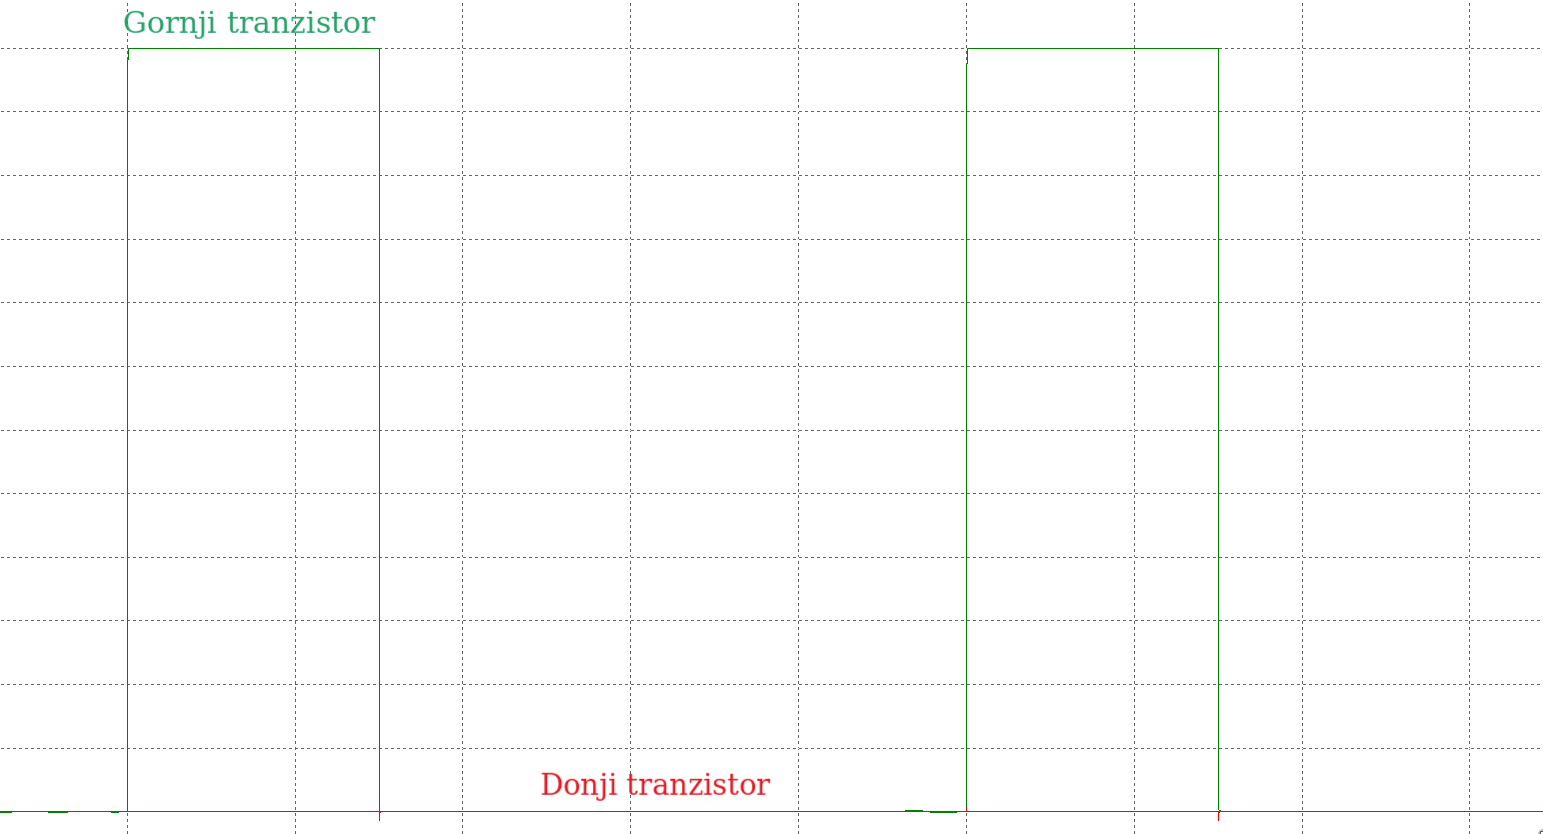
\includegraphics[width=0.95\textwidth]{Figures/hard_chopping1.png}
		      \caption{Glatko preklapanje u alatu LTspice}
		      \label{fig:hard_chopping}
	      \end{figure}

	\item \textbf{Komplementarni signal PWM-a:}

	      Isti scenarij kao i na prošlom primjeru, ali na nizak signal PWM-a struja
	      recirkulira kroz tranzistor $S_2$ a kada je on nizak, uključuje se donja
	      sklopka u istom polumostu što se može vidjeti na slici \ref{fig:soft_chopping}.
	      Kada se zeleni signal na tranzistoru $S_1$ spusti u nisko stanje, crveni signal
	      na tranzistoru $S_2$ sa malom stankom podigne se u visoko stanje. Ova mala
	      stanka naziva se mrtvo vrijeme (eng. \textit{dead time}) i sprječava kratki
	      spoj na polumostu (eng. \textit{shoot-through}). Uključivanjem donjeg
	      tranzistora na ovaj način postiže se da struja recirkulira kroz tranzistor
	      \cite{TI2015}. \todo[inline]{fale osi na slici}
	      \begin{figure}[h!]
		      \centering
		      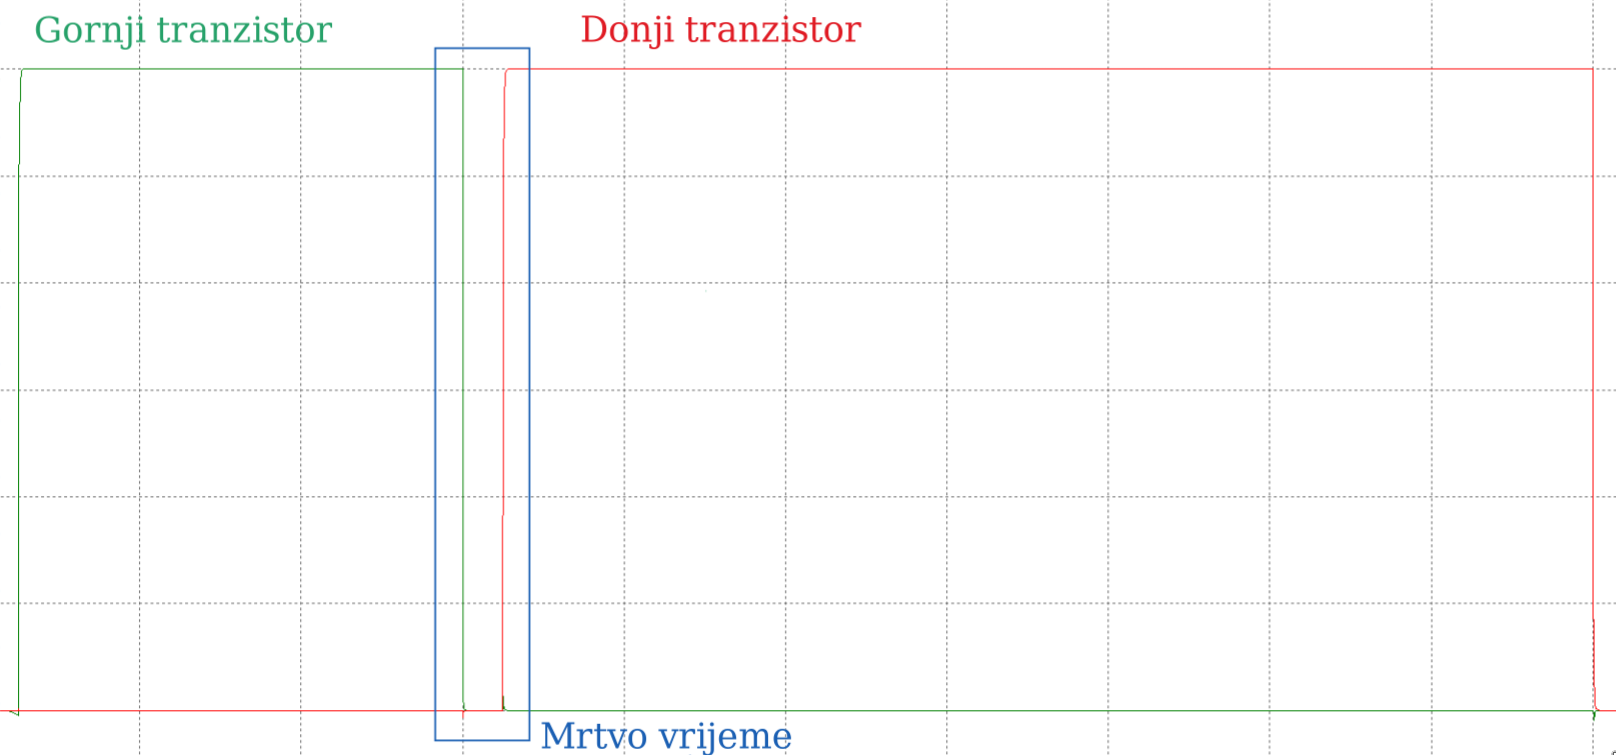
\includegraphics[width=0.95\textwidth]{Figures/soft_chopping.png}
		      \caption{Komplementarni signal PWM-a u alatu LTspice}
		      \label{fig:soft_chopping}
	      \end{figure}

\end{itemize}

Izbor metode upravljanja strujom u ciklusu PWM-a utječe na dinamiku struje i
razinu elektromagnetskih smetnji. Od metode oštrog preklapanja do metode
komplementarnog signala PWM-a postepena je gradacija sa većih gubitaka na manje
gubitke energije. Isto tako složenost izvedbe raste tim redoslijedom. Na
slikama \ref{fig:hard_soft_current} mogu se vidjeti valni oblici struje kroz
zavojnice u metodama glatkog preklapanja i komplementarnog signala PWM-a. Slika
\ref{fig:hard_current} prikazuje brži pad struje pri niskom signalu PWM-a te
samim time i nižu prosječnu struju od struje pri metodi komplementarnog signala
PWM-a prikazane na slici \ref{fig:soft_current}.
\begin{figure}[h!]
	\begin{subfigure}[b]{0.48\textwidth}
		\centering
		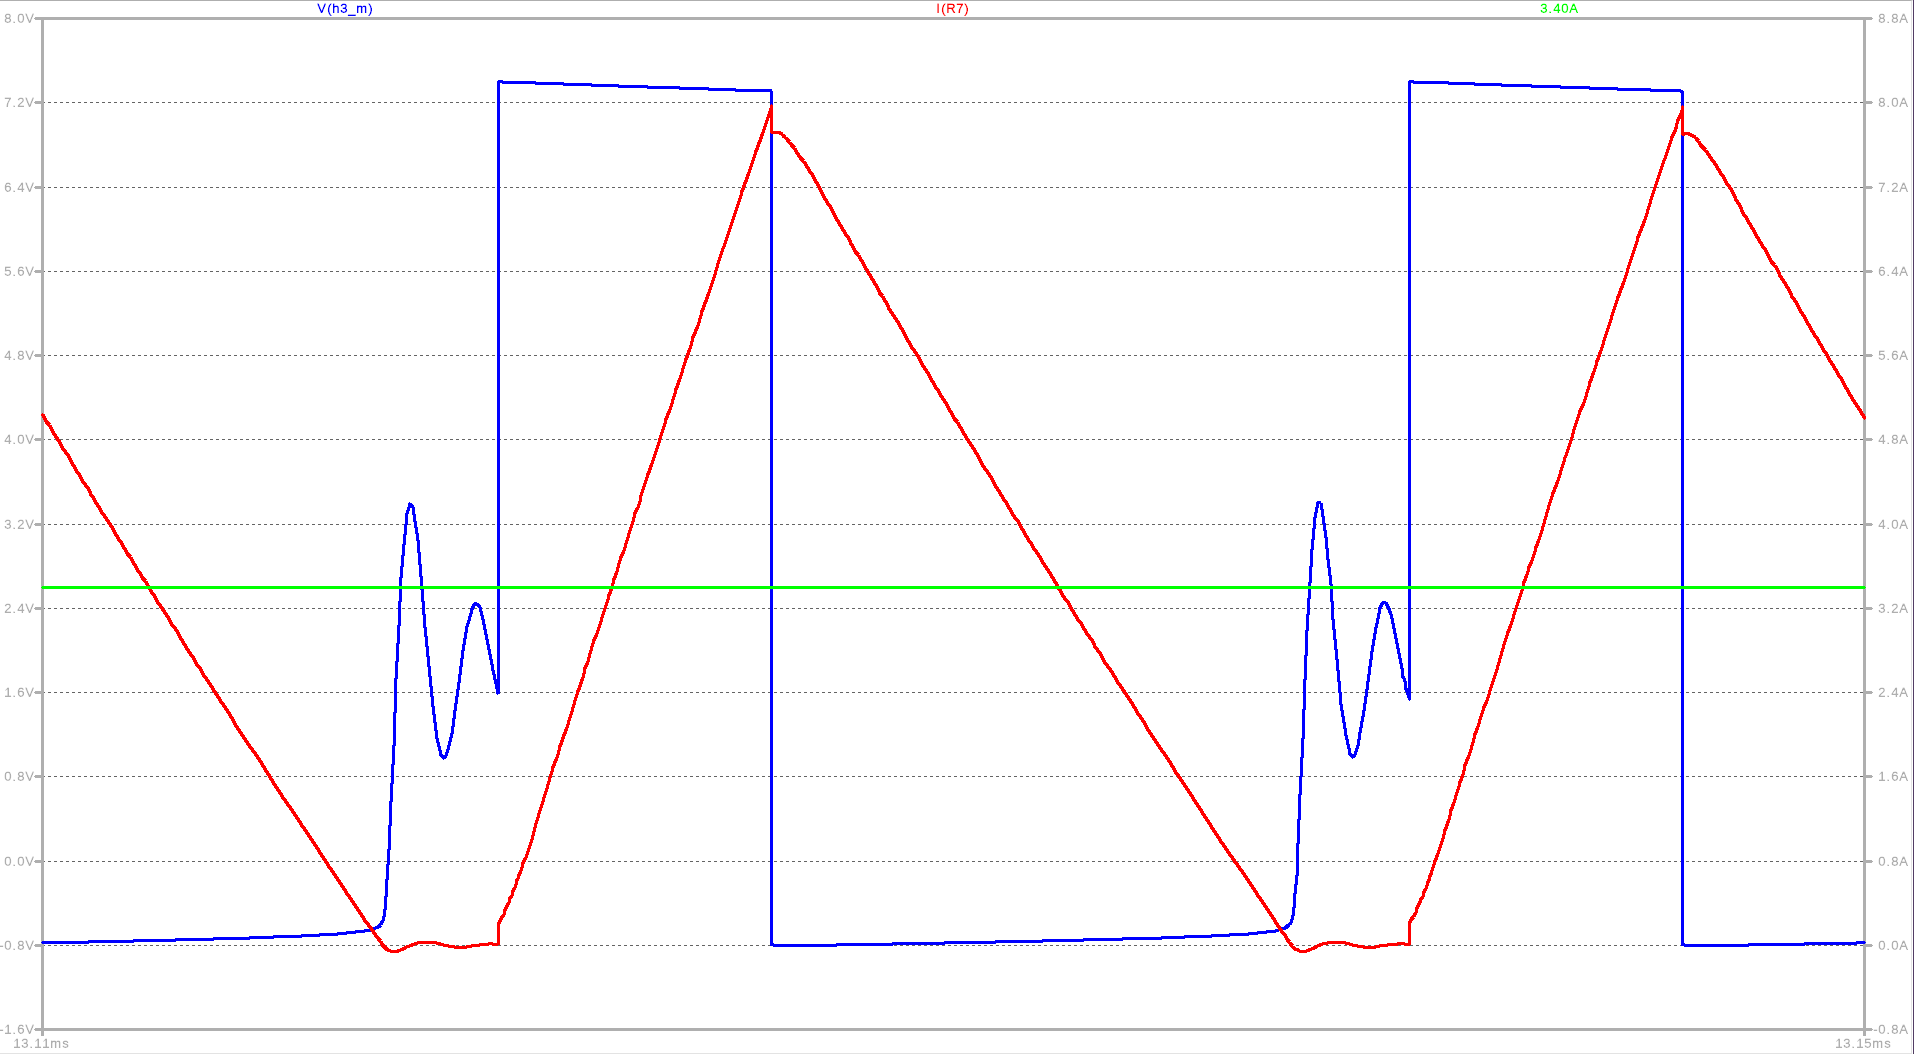
\includegraphics[width=\textwidth]{Figures/soft_chopping_new.png}
		\caption{Glatko preklapanje}
		\label{fig:hard_current}
	\end{subfigure}
	\begin{subfigure}[b]{0.48\textwidth}
		\centering
		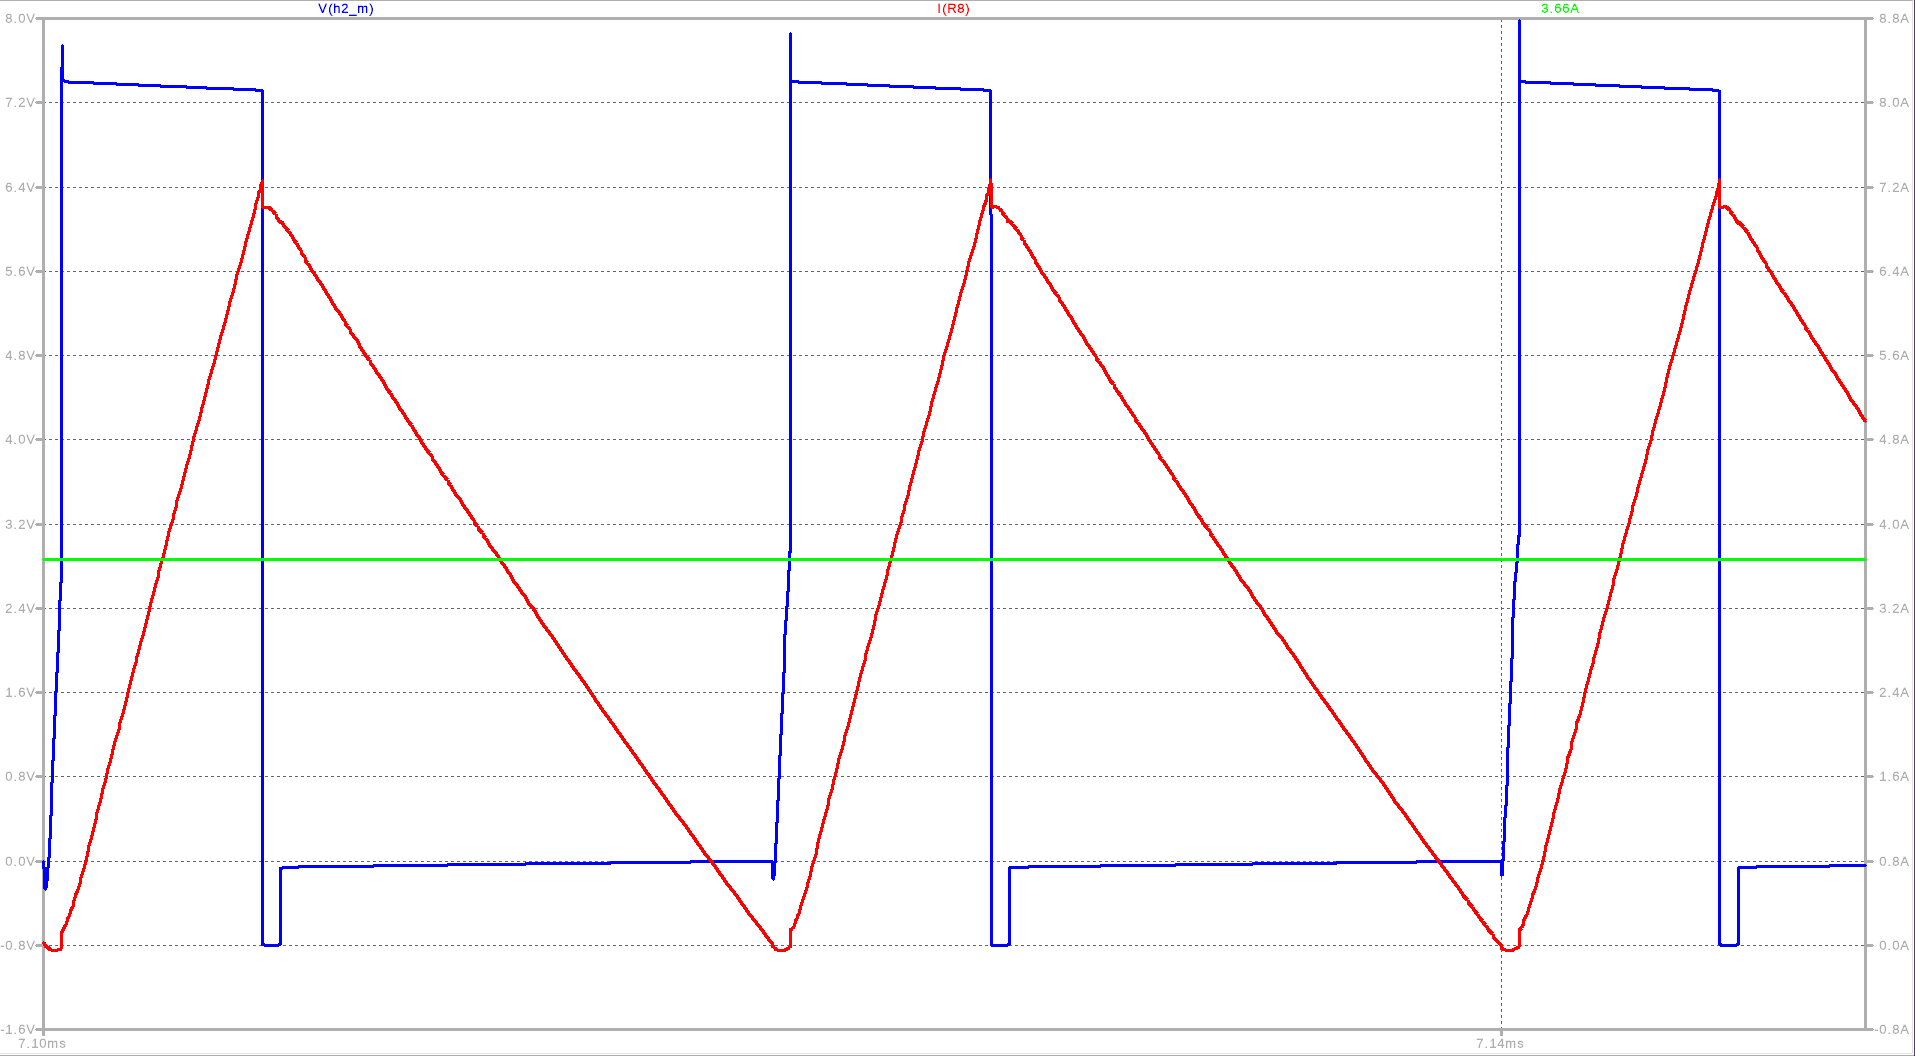
\includegraphics[width=\textwidth]{Figures/comp_pwm_new.png}
		\caption{komplementarni signal PWM-a}
		\label{fig:soft_current}
	\end{subfigure}
	\caption{
		\begin{tabular}[t]{@{}l l@{}}
			\textcolor{red}{\rule{1ex}{1ex}}   & Valni oblik struje \\
			\textcolor{green}{\rule{1ex}{1ex}} & Prosječna struja   \\
			\textcolor{blue}{\rule{1ex}{1ex}}  & Valni oblik napona \\
		\end{tabular}
	}	\label{fig:hard_soft_current}
\end{figure}
\newpage

\section{Detekcija položaja rotora s pomoću PEMS-a}

U sustavima bez osjetila, informacija o položaju rotora dobiva se mjerenjem
napona protuelektromotorne sile na neopterećenoj fazi.

U konfiguraciji sa zvjezdastim spojem, PEMS se mjeri u odnosu na potencijal
zvjezdišta. Budući da zvjezdište motora najčešće nije fizički dostupno za
mjerenje, njegov se potencijal mora rekonstruirati. To se postiže stvaranjem
virtualnog zvjezdišta (slika \ref{fig:rekonstrukcija}). Tri otpornika jednakog,
visokog otpora $R_v$ spajaju se u zvijezdu, pri čemu je svaki otpornik spojen
na po jednu fazu motora. Zajednička točka ta tri otpornika stvara virtualno
zvjezdište $V_{virtual}$ čiji je potencijal jednak aritmetičkoj sredini napona
sve tri faze. Taj se stabilni referentni napon tada koristi za usporedbu s
naponom neopterećene faze \cite{ST_AN1946}.

\begin{figure}[h]
	\centering
	\resizebox{\textwidth}{!}{
		\begin{circuitikz}[european, cute inductors]
			\draw[R={$R_a$},/tikz/circuitikz/bipoles/length=1.1cm](13.0,-6.0)to(14.5,-6.0);
			\draw[R={$R_b$},/tikz/circuitikz/bipoles/length=1.1cm](13.0,-8.0)to(14.5,-8.0);
			\draw[R={$R_c$},/tikz/circuitikz/bipoles/length=1.1cm](13.0,-10.0)to(14.5,-10.0);
			\draw[short={}](14.5,-6.0)to(14.5,-6.0);
			\draw[short={}](13.0,-10.0)to(13.0,-12.0);
			\draw[short={}](13.0,-12.0)to(13.0,-12.0);
			\draw[short={}](13.0,-8.0)to(11.5,-8.0);
			\draw[short={}](11.5,-8.0)to(11.5,-8.0);
			\draw[short={}](11.5,-8.0)to(11.5,-12.0);
			\draw[short={}](13.0,-6.0)to(10.0,-6.0);
			\draw[short={}](10.0,-6.0)to(10.0,-12.0);
			\draw[short={}](10.0,-12.0)to(10.0,-12.0);
			\draw[R={$R_v$},/tikz/circuitikz/bipoles/length=1.1cm](10.0,-12.0)to(10.0,-13.5);
			\draw[R={$R_v$},/tikz/circuitikz/bipoles/length=1.1cm](11.5,-12.0)to(11.5,-13.5);
			\draw[R={$R_v$},/tikz/circuitikz/bipoles/length=1.1cm](13.0,-12.0)to(13.0,-13.5);
			\draw[short={}](10.0,-13.5)to(10.0,-14.0);
			\draw[short={}](10.0,-14.0)to(10.0,-14.0);
			\draw[short={}](10.0,-14.0)to(13.0,-14.0);
			\draw[short={}](13.0,-13.5)to(13.0,-14.0);
			\draw[short={}](13.0,-14.0)to(13.0,-14.0);
			\draw[short={}](11.5,-13.5)to(11.5,-14.0);
			\draw node[circ] (S38) at (11.5, -14.0) {} node[anchor=south] at ([yshift=-0.6cm]S38.text){$V_{virtual}$};
			\ctikzset{tripoles/mos style/arrows}
			\draw node[nmos,scale=0.59,xscale=1,yscale=1,rotate=0](Q40) at (8.0,-4.5) {} node[anchor=west,scale=0.9] at (Q40.text){}
			node[left=5mm,scale=0.9] at (Q40.text) {$S_{5}$};
			\draw[short](Q40.C)to(8.0,-4.0);
			\draw[short](Q40.E)to(8.0,-5.0);
			\ctikzset{tripoles/mos style/arrows}
			\draw node[nmos,scale=0.59,xscale=1,yscale=1,rotate=0](Q41) at (8.0,-11.0) {} node[anchor=west,scale=0.9] at (Q41.text){}
			node[left=5mm,scale=0.9] at (Q41.text) {$S_{6}$};
			\draw[short](Q41.C)to(8.0,-10.5);
			\draw[short](Q41.E)to(8.0,-11.5);
			\ctikzset{tripoles/mos style/arrows}
			\draw node[nmos,scale=0.59,xscale=1,yscale=1,rotate=0](Q42) at (5.0,-11.0) {} node[anchor=west,scale=0.9] at (Q42.text){}
			node[left=5mm,scale=0.9] at (Q42.text) {$S_{4}$};
			\draw[short](Q42.C)to(5.0,-10.5);
			\draw[short](Q42.E)to(5.0,-11.5);
			\ctikzset{tripoles/mos style/arrows}
			\draw node[nmos,scale=0.59,xscale=1,yscale=1,rotate=0](Q43) at (5.0,-4.5) {} node[anchor=west,scale=0.9] at (Q43.text){}
			node[left=5mm,scale=0.9] at (Q43.text) {$S_{3}$};
			\draw[short](Q43.C)to(5.0,-4.0);
			\draw[short](Q43.E)to(5.0,-5.0);
			\ctikzset{tripoles/mos style/arrows}
			\draw node[nmos,scale=0.59,xscale=1,yscale=1,rotate=0](Q44) at (2.0,-4.5) {} node[anchor=west,scale=0.9] at (Q44.text){}
			node[left=5mm,scale=0.9] at (Q44.text) {$S_{1}$};
			\draw[short](Q44.C)to(2.0,-4.0);
			\draw[short](Q44.E)to(2.0,-5.0);
			\ctikzset{tripoles/mos style/arrows}
			\draw node[nmos,scale=0.59,xscale=1,yscale=1,rotate=0](Q45) at (2.0,-11.0) {} node[anchor=west,scale=0.9] at (Q45.text){}
			node[left=5mm,scale=0.9] at (Q45.text) {$S_{2}$};
			\draw[short](Q45.C)to(2.0,-10.5);
			\draw[short](Q45.E)to(2.0,-11.5);
			\draw[short={}](2.0,-5.0)to(2.0,-5.0);
			\draw[short={}](2.0,-5.0)to(2.0,-10.5);
			\draw[short={}](5.0,-5.0)to(5.0,-10.5);
			\draw[short={}](8.0,-5.0)to(8.0,-10.5);
			\draw node[ground] (G50) at (2.0, -12.5) {} node[anchor=north] at ([yshift=-0.6cm]G50.text){};
			\draw node[ground] (G51) at (5.0, -12.5) {} node[anchor=north] at ([yshift=-0.6cm]G51.text){};
			\draw node[ground] (G52) at (8.0, -12.5) {} node[anchor=north] at ([yshift=-0.6cm]G52.text){};
			\draw(2.0,-3.5)to(2.0,-3.5) node[vcc] {};
			\draw(5.0,-3.5)to(5.0,-3.5) node[vcc] {};
			\draw(8.0,-3.5)to(8.0,-3.5) node[vcc] {};
			\draw[short={}](2.0,-3.5)to(2.0,-4.0);
			\draw[short={}](5.0,-3.5)to(5.0,-4.0);
			\draw[short={}](8.0,-3.5)to(8.0,-4.0);
			\draw[short={}](8.0,-11.5)to(8.0,-12.5);
			\draw[short={}](5.0,-11.5)to(5.0,-12.5);
			\draw[short={}](2.0,-11.5)to(2.0,-12.5);
			\draw[crossing={},/tikz/circuitikz/bipoles/length=1.1cm](4.5,-6.0)to(5.5,-6.0);
			\draw[crossing={},/tikz/circuitikz/bipoles/length=1.1cm](7.5,-6.0)to(8.5,-6.0);
			\draw[crossing={},/tikz/circuitikz/bipoles/length=1.1cm](7.5,-8.0)to(8.5,-8.0);
			\draw[short={}](2.0,-6.0)to(4.5,-6.0);
			\draw[short={}](4.5,-6.0)to(4.5,-6.0);
			\draw[short={}](5.5,-6.0)to(7.5,-6.0);
			\draw[short={}](8.5,-6.0)to(10.0,-6.0);
			\draw[short={}](5.0,-8.0)to(7.5,-8.0);
			\draw[short={}](8.5,-8.0)to(8.5,-8.0);
			\draw[crossing={},/tikz/circuitikz/bipoles/length=1.1cm](9.5,-8.0)to(10.5,-8.0);
			\draw[crossing={},/tikz/circuitikz/bipoles/length=1.1cm](9.5,-10.0)to(10.5,-10.0);
			\draw[crossing={},/tikz/circuitikz/bipoles/length=1.1cm](11.0,-10.0)to(12.0,-10.0);
			\draw[short={}](8.0,-10.0)to(9.5,-10.0);
			\draw[short={}](10.5,-10.0)to(11.0,-10.0);
			\draw[short={}](12.0,-10.0)to(13.0,-10.0);
			\draw[short={}](13.0,-10.0)to(13.0,-10.0);
			\draw[short={}](8.5,-8.0)to(9.5,-8.0);
			\draw[short={}](10.5,-8.0)to(11.5,-8.0);
			\draw node[circ] (S80) at (10.0, -6.0) {} node[anchor=south] at ([yshift=-0.6cm]S80.text){};
			\draw node[circ] (S81) at (11.5, -8.0) {} node[anchor=south] at ([yshift=-0.6cm]S81.text){};
			\draw node[circ] (S82) at (13.0, -10.0) {} node[anchor=south] at ([yshift=-0.6cm]S82.text){};
			\draw[D={},/tikz/circuitikz/bipoles/length=1.1cm](2.5,-5.0)to(2.5,-4.0);
			\draw[D={},/tikz/circuitikz/bipoles/length=1.1cm](2.5,-11.5)to(2.5,-10.5);
			\draw[D={},/tikz/circuitikz/bipoles/length=1.1cm](5.5,-11.5)to(5.5,-10.5);
			\draw[D={},/tikz/circuitikz/bipoles/length=1.1cm](5.5,-5.0)to(5.5,-4.0);
			\draw[D={},/tikz/circuitikz/bipoles/length=1.1cm](8.5,-5.0)to(8.5,-4.0);
			\draw[D={},/tikz/circuitikz/bipoles/length=1.1cm](8.5,-11.5)to(8.5,-10.5);
			\draw[short={}](5.0,-10.5)to(5.5,-10.5);
			\draw[short={}](5.0,-11.5)to(5.5,-11.5);
			\draw[short={}](2.0,-10.5)to(2.5,-10.5);
			\draw[short={}](2.0,-11.5)to(2.5,-11.5);
			\draw[short={}](2.0,-4.0)to(2.5,-4.0);
			\draw[short={}](2.0,-5.0)to(2.5,-5.0);
			\draw[short={}](2.5,-4.5)to(2.5,-4.5);
			\draw[short={}](5.0,-4.0)to(5.5,-4.0);
			\draw[short={}](5.0,-5.0)to(5.5,-5.0);
			\draw[short={}](8.0,-4.0)to(8.5,-4.0);
			\draw[short={}](8.0,-5.0)to(8.5,-5.0);
			\draw[short={}](8.0,-10.5)to(8.5,-10.5);
			\draw[short={}](8.0,-11.5)to(8.5,-11.5);
			\draw[short={}](8.5,-11.5)to(8.5,-11.5);
			\draw[L={$L_a$},/tikz/circuitikz/bipoles/length=1.1cm](15.0,-6.0)to(16.0,-6.0);
			\draw[L={$L_b$},/tikz/circuitikz/bipoles/length=1.1cm](15.0,-8.0)to(16.0,-8.0);
			\draw[L={$L_c$},/tikz/circuitikz/bipoles/length=1.1cm](15.0,-10.0)to(16.0,-10.0);
			\draw[V<={$e_a$},/tikz/circuitikz/bipoles/length=1.1cm](16.5,-6.0)to(17.5,-6.0);
			\draw[V<={$e_b$},/tikz/circuitikz/bipoles/length=1.1cm](16.5,-8.0)to(17.5,-8.0);
			\draw[V<={$e_c$},/tikz/circuitikz/bipoles/length=1.1cm](16.5,-10.0)to(17.5,-10.0);
			\draw[short={}](17.5,-6.0)to(18.0,-6.0);
			\draw[short={}](18.0,-6.0)to(18.0,-10.0);
			\draw[short={}](17.5,-10.0)to(18.0,-10.0);
			\draw[short={}](17.5,-8.0)to(18.0,-8.0);
			\draw node[circ] (S96) at (18.0, -8.0) {} node[anchor=south] at ([yshift=-0.6cm]S96.text){$V_{neutral}$};
			\draw[short={}](14.5,-6.0)to(15.0,-6.0);
			\draw[short={}](16.0,-6.0)to(16.5,-6.0);
			\draw[short={}](16.0,-8.0)to(16.5,-8.0);
			\draw[short={}](16.0,-10.0)to(16.5,-10.0);
			\draw[short={}](14.5,-10.0)to(15.0,-10.0);
			\draw[short={}](14.5,-8.0)to(15.0,-8.0);
		\end{circuitikz}
	}
	\caption{Rekonstrukcija zvjezdišta}
	\label{fig:rekonstrukcija}
\end{figure}

Za preciznu detekciju trenutka u kojem protuelektromotorna sila prolazi kroz
nulu koristi se sklop komparatora, no točna implementacija ovisi o metodi
uzorkovanja koja je usko vezana za signal PWM-a. "Klasična" metoda uzorkuje
napon faze za vrijeme visokog stanja signala PWM-a, što omogućuje postizanje
100\% radnog ciklusa, ali zahtijeva filtriranje signala i referentnog napona
zbog šuma uzrokovanog sklapanjem tranzistora vidljivog na slici
\ref{fig:pwm_sum} \cite{ST_AN1946}.

\begin{figure}[h!]
	\centering
	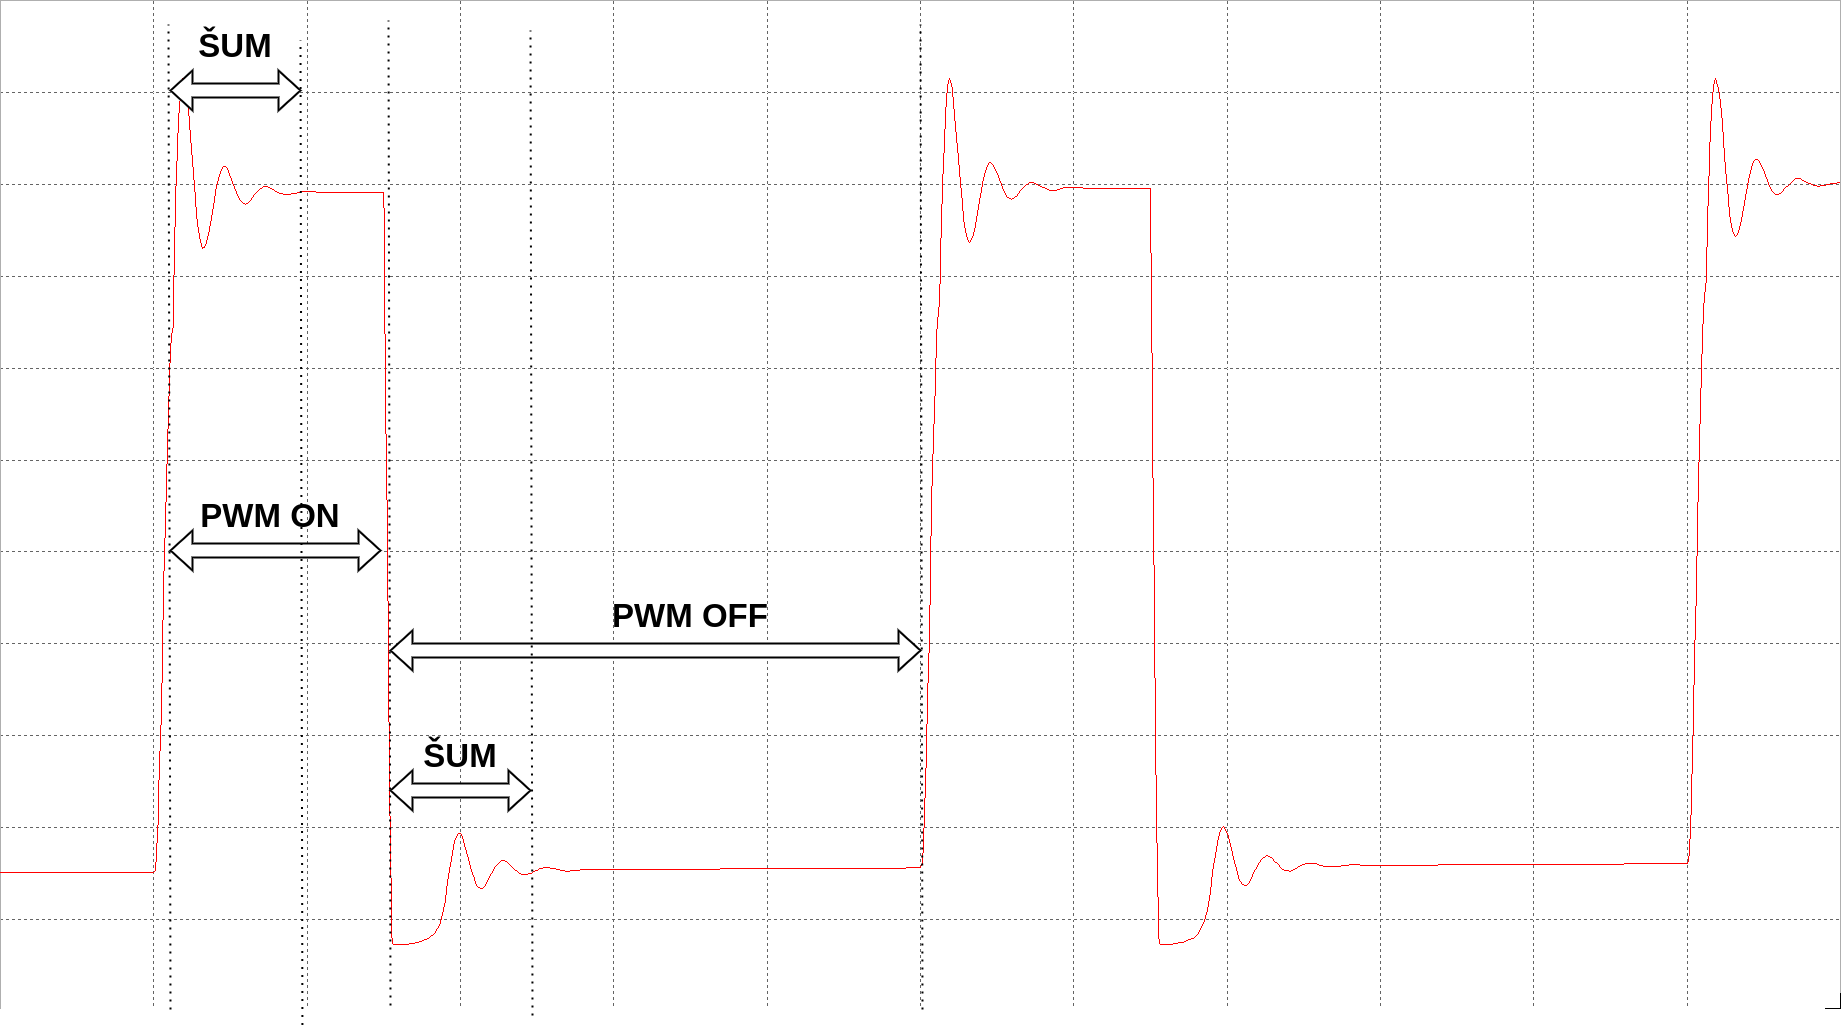
\includegraphics[width=0.95\textwidth]{Figures/pwm_sum.png}
	\caption{Prikaz napona na neopterećenoj fazi u alatu LTspice}
	\label{fig:pwm_sum}
\end{figure}

Alternativna i cjenovno učinkovitija strategija je uzorkovanje na kraju niskog
stanja signala PWM-a. U tom intervalu, kada struja recirkulira kroz diodu ili
tranzistor, mjerenje je jednostavnije i otpornije na šum jer se potencijal
zvjezdišta može smatrati uzemljenim, no nedostatak je nemogućnost postizanja
100\% radnog ciklusa \label{text:pwm_off}. Postoje i hibridne metode koje
kombiniraju ova dva pristupa kako bi iskoristile prednosti obiju strategija
ovisno o brzini i opterećenju motora \cite{ST_AN1946}.

Ovaj događaj prolaska kroz nulu događa se točno na polovici trajanja jednog
komutacijskog koraka kao što se može vidjeti na slici \ref{fig:pwm_drive}.
Drugim riječima, od trenutka detekcije presijecanja nule do idealnog trenutka
za sljedeću komutaciju potrebno je pričekati vrijeme koje odgovara zakretu od
30 električnih stupnjeva.

\begin{figure}[h!]
	\centering
	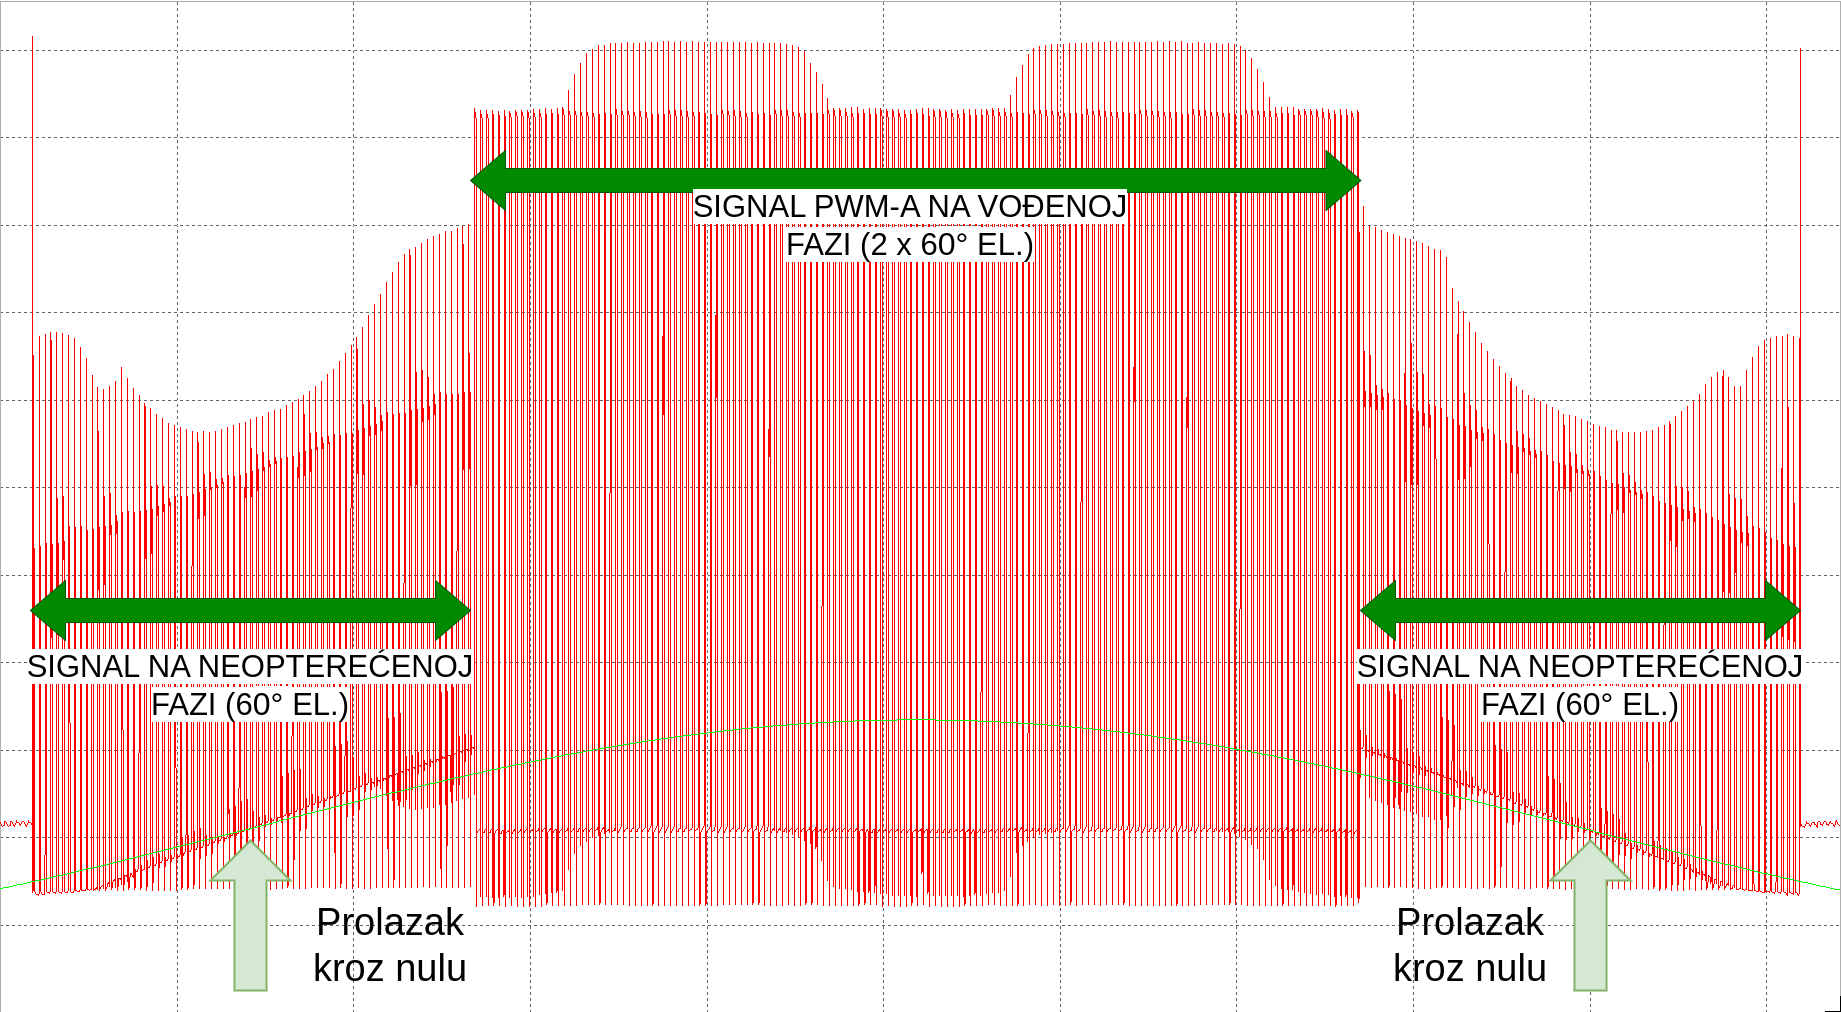
\includegraphics[width=0.95\textwidth]{Figures/pwm_drive_deg.png}
	\caption{Prikaz signala PWM-a na jednoj fazi u alatu LTspice}
	\label{fig:pwm_drive}
\end{figure}

\newpage

\section{Faze pokretanja i rada motora}

Pokretanje motora bez osjetila ne može se izvesti isključivo detektiranjem
PEMS-a jer nije prisutan pri mirovanju i vrlo malim brzinama ili je preslab za
detekciju. Potrebno je motor dovesti do stanja gdje može očitavati PEMS.

Prije pokretanja, položaj rotora je nepoznat. Kako bi se postavio u poznati
početni položaj, na kratko se vrijeme uključe dva fazna namotaja. To stvara
statično magnetsko polje koje poravnava rotor u određenom smjeru. Ova faza se
naziva poravnanje (eng. \textit{alignment}). Nakon poravnanja, motor se pokreće
u otvorenoj petlji (eng. \textit{open-loop}). Sklop ESC forsira komutaciju
namotaja prema unaprijed definiranom, postupno rastućem vremenskom slijedu, bez
ikakve povratne informacije o stvarnom položaju. Cilj je ubrzati motor do
brzine na kojoj će inducirani PEMS biti dovoljno velik za pouzdanu detekciju.
Kada brzina dosegne prag na kojem detekcija prolaska kroz nulu postaje
pouzdana, sustav prelazi u rad sa zatvorenom petljom (eng.
\textit{closed-loop}). Od ovog trenutka, komutacija se više ne temelji na
fiksnom vremenu, već je sinkronizirana sa stvarnim položajem rotora
detektiranim prolaskom PEMS-a kroz nulu \cite{Recasens2021}.

\section{Model regulacije brzine}
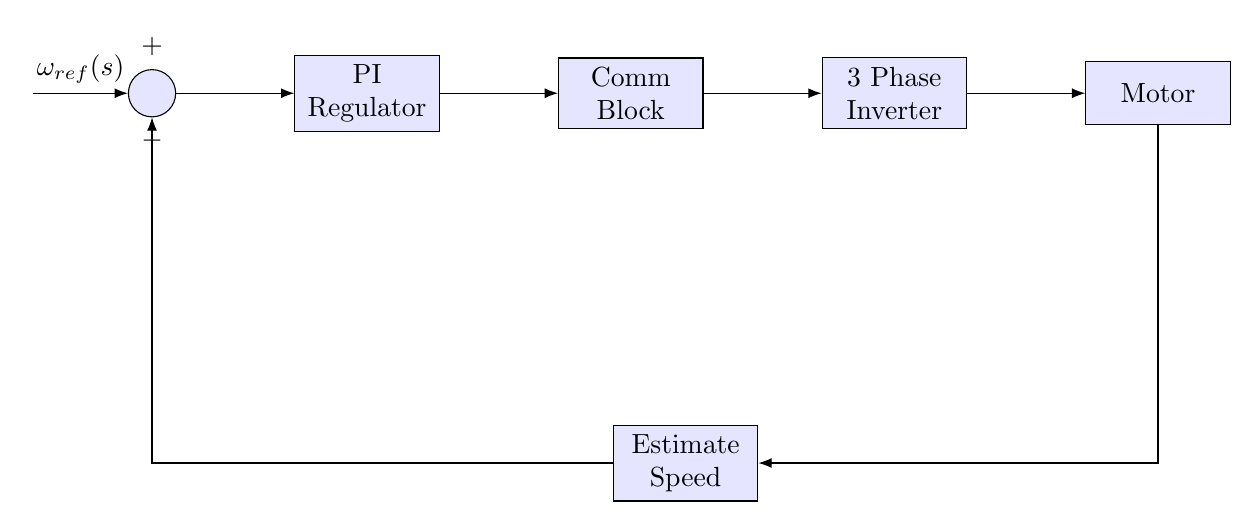
\begin{tikzpicture}[
		auto,
		node distance=1.8cm and 1.5cm, % Reduced distance between nodes (vertical and horizontal)
		>=Latex, % Use LaTeX-style arrows
		block/.style={
				draw,
				rectangle,
				fill=blue!10,
				minimum height=0.8cm, % Slightly reduced height
				minimum width=1.8cm, % Reduced width
				text width=1.6cm, % Ensures text wraps if needed, corresponds to minimum width
				align=center
			},
		sum/.style={
				draw,
				circle,
				fill=blue!10,
				minimum size=0.6cm, % Slightly reduced size
				node distance=1.2cm % Reduced distance for sum node
			},
		io/.style={
				coordinate
			},
		pinstyle/.style={
				pin edge={to-,thin,black}
			}
	]
	% Nodes
	\node[io, name=input] {};
	\node[sum, right=of input, name=sum] {};
	\node[block, right=of sum, name=pi_regulator] {PI Regulator};
	\node[block, right=of pi_regulator, name=comm_block] {Comm Block};
	\node[block, right=of comm_block, name=inverter] {3 Phase Inverter};
	\node[block, right=of inverter, name=motor] {Motor};
	%\node[io, right=of motor, name=output_motor] {}; % Output from motor
	\node[block, below=of motor,xshift=-6.0cm, yshift=-2.0cm, name=estimate_speed] {Estimate Speed}; % Adjusted yshift

	% Paths
	\draw[->] (input) -- node[above] {$\omega_{ref}(s)$} (sum);
	\draw[->] (sum) -- (pi_regulator);
	\draw[->] (pi_regulator) -- (comm_block);
	\draw[->] (comm_block) -- (inverter);
	\draw[->] (inverter) -- (motor);
	%\draw[->] (motor) -- (output_motor);
	\draw[->] (motor) |- (estimate_speed);
	\draw[->] (estimate_speed) -| (sum);

	% Summing Junction Signs
	\node at (sum.north) [above=0.05cm] {$+$}; % Slightly adjusted for smaller sum node
	\node at (sum.west) [left=0.05cm] {};
	\node at (sum.south) [below=0.05cm] {$-$};
\end{tikzpicture}%-------------------------------------------------------------------------------
\chapter{Eksperimentalni postav}
\label{pog:postav}

Kako bi se provela validacija teorijskih koncepata i testirala implementacija
algoritma za upravljanje brzinom vrtnje, sastavljen je eksperimentalni postav.
Ovaj postav objedinjuje sve sklopovske i programske komponente potrebne za
pogon i analizu rada istosmjernog motora bez četkica. U nastavku su opisane
komponente korištene u radu.

\section{Elektronički sklop za upravljanje brzinom}
\label{sec:esc}

Središnji element eksperimentalnog postava je elektronički sklop za upravljanje
brzinom motora. On objedinjuje digitalnu upravljačku logiku i pogonski sklop na
dvije odvojene tiskane pločice (eng. \textit{Printed Circuit Board, PCB}).

Digitalna upravljačka logika implementirana je na razvojnoj pločici
\textit{Nucleo G071RB}, čija je središnja komponenta mikrokontroler
\textit{STM32G071RB}. Njegova zadaća je izvršavanje upravljačkog algoritma što
obuhvaća generiranje signala pulsno-širinske modulacije (eng.
\textit{Pulse-Width Modulation}, PWM) za upravljanje tranzistorima snage te
akviziciju i obradu signala protuelektromotorne sile za određivanje položaja
rotora.

Pogonski sklop, zadužen za isporuku energije motoru, realiziran je na zasebnoj,
ručno zalemljenoj tiskanoj pločici\footnote{Dizajn tiskane pločice za potrebe
	ovog rada ustupio je Boris Šnajder}. Njegovu osnovu čine tri polumosta koja
pogone tri faze motora. Svaki polumost sastoji se od para komplementarnih
tranzistora snage tipa MOSFET. Na istoj pločici nalaze se i sklopovi za
kondicioniranje signala koji obavljaju filtriranje i prilagodbu naponskih
razina faznih napona. Sklop komparatora koristi se za detekciju trenutka
prolaska signala PEMS-a kroz referentni napon virtualnog zvjezdišta.
\missingfigure{slika esc}

\section{Elektromotor \textit{A2212/13T  1000KV}}
\label{sec:motor}

U eksperimentu je korišten komercijalno dostupan trofazni istosmjerni motor bez
četkica modela \textit{A2212/13T}. Oznaka \textit{A2212/13T} odnosi se na
njegove konstrukcijske značajke. Oznaka \textit{2212} specificira dimenzije
statora: promjer od 22 mm i visinu od 12 mm. Motor ima 14 magnetskih polova na
rotoru i 12 utora na statoru, što odgovara uobičajenoj konfiguraciji 14P12N za
ovu vrstu motora. Riječ je o vanjskom motoru konstante brzine od 1000 KV, što
specificira da motor teoretski, u neopterećenom stanju, postiže brzinu vrtnje
od 1000 okretaja u minuti za svaki volt napona napajanja. Oznaka \textit{13T}
odnosi se na broj namotaja na svakom polu statora, što utječe na njegove
momentne i brzinske karakteristike. \missingfigure{slika motora}

\section{Enkoder}
\label{sec:enkoder}

Za precizno mjerenje stvarne brzine vrtnje i položaja rotora motora korišten je
apsolutni magnetski enkoder \textit{CUI Devices AMT223C-V}. Iako se primarni
algoritam upravljanja opisan u ovom radu temelji na metodi bez osjetila
položaja, enkoder je u eksperimentalnom postavu imao ulogu referentnog mjernog
uređaja. Podaci dobiveni s enkodera služili su za praćenje kuta između statora
i rotora, za praćenje trajanja pojedinog koraka te za praćenje trenutaka
detektiranih prolazaka kroz nulu. \missingfigure{slika enkodera}

Kako bi se osigurala mehanička stabilnost i pouzdano centriranje enkodera na
osovinu motora, pomoću tehnologije 3D tiska izrađeno je prilagođeno kućište
koje fiksira enkoder i motor u koaksijalan položaj. \missingfigure{slika
	enkodera na motoru + kuciste}

\section{Mjerni instrumenti}
\label{sec:mjerni_instrumenti}

Tijekom razvoja, testiranja i analize sustava korištena je standardna
laboratorijska mjerna oprema. Kao izvor napajanja za elektronički sklop i motor
služilo je laboratorijsko napajanje, koje je osiguravalo stabilan i podesiv
istosmjerni napon. Za analizu signala korišteni su digitalni osciloskop i
logički analizator. Digitalnim osciloskopom obavljena je vizualizacija i
mjerenje analognih signala, kao što su valni oblici faznih napona, signali
protuelektromotorne sile i izlazi komparatora. Za praćenje i analizu digitalnih
signala upotrijebljen je logički analizator \textit{Saleae}, primarno za
dekodiranje podataka o položaju s enkodera te praćenje pomoćnih signala tijekom
otklanjanja pogrešaka. Uz navedene instrumente, digitalni multimetar korišten
je za osnovna mjerenja istosmjernog napona, struje i otpora prilikom
sastavljanja i provjere ispravnosti elektroničkog sklopa.

\section{Programska podrška}
\label{sec:programska_podrska}

Uz sklopovske komponente i mjerne instrumente, u radu je korištena i programska
podrška za simulaciju elektroničkih krugova, za obradu i vizualizaciju mjernih
podataka te za pojednostavljeno upravljanje brzinom vrtnje. U fazi istraživanja
teme, ponašanje ključnih dijelova pogonskog sklopa simulirano je u alatu
\textit{LTspice}. To je omogućilo bolje razumijevanje koncepata poput ponašanja
struje pri različitim tehnikama primjene PWM-a na upravljanje \ref{sss:pwm}.

Podaci prikupljeni s enkodera su uvezeni, obrađeni i vizualizirani pomoću
programskog paketa \textit{MATLAB}. Obrada u \textit{MATLAB}-u omogućila je
uvid u promjene kuta kroz vrijeme, trajanje svakog pojedinačnog koraka,
trenutke detektiranog prolaska kroz nulu te odziv brzine kroz vrijeme što je
olakšalo i ubrzalo proces razvoja algoritma.

Za upravljanje brzinom vrtnje korištena je jednostavna skripta napisana u
jeziku Python za slanje tražene brzine na sklop ESC te primanje trenutne brzine
rotora preko sučelja UART.

%-------------------------------------------------------------------------------
\chapter{Implementacija}
\label{pog:implementacija}

Ovo poglavlje opisuje programsku implementaciju sustava za upravljanje brzinom
vrtnje motora BLDC bez osjetila položaja. Prikazana je arhitektura programskog
rješenja, konfiguracija korištenih perifernih jedinica mikrokontrolera
\texttt{STM32G071RB} te programska realizacija algoritma za upravljanje i
regulaciju brzine. Implementacija se temelji na teorijskim konceptima opisanim
u prethodnim poglavljima i odnosi se na sklopovlje korišteno u eksperimentalnom
postavu.

\section{Arhitektura programskog rješenja}
\label{sec:arhitektura_rjesenja}

Programsko rješenje implementirano je izravno na sklopovlju (eng.
\textit{bare-metal}), bez korištenja operacijskog sustava. Cjelokupna
arhitektura temelji se na beskonačnoj petlji unutar glavne funkcije te na
sustavu prekida za obradu vremenski kritičnih događaja.

Sustav je vođen prekidima (eng. \textit{interrupt-driven}). Operacije koje
zahtijevaju precizno vremensko izvršavanje, poput generiranja signala PWM-a,
detekcije protuelektromotorne sile i same komutacije, iniciraju se i obrađuju
unutar prekidnih rutina hardverskih tajmera. Glavna programska petlja služi za
obradu događaja koji su signalizirani iz prekidnih rutina putem globalnih
zastavica (eng. \textit{flags}). Ovakav pristup minimizira vrijeme provedeno
unutar prekidnih rutina i omogućuje izvršavanje složenije obrade podataka u
glavnom dijelu programa.

Rad sustava slijedi logičan tijek kroz nekoliko faza, od pokretanja do rada u
ustaljenom stanju:
\begin{itemize}
	\item \textbf{Mirovanje:} Početno stanje u kojem motor nije aktivan.
	\item \textbf{Poravnanje (eng. \textit{Alignment}):} Prvi korak pri pokretanju, gdje se izvršavaju dva relativno dugačka koraka komutacije kako bi se rotor postavio u poznati početni položaj.
	\item \textbf{Rad u otvorenoj petlji (eng. \textit{Open-loop}):} Faza ubrzavanja motora u kojoj se komutacija izvodi prisilno, prema unaprijed definiranoj vremenskoj sekvenci i bez povratne veze o stvarnom položaju rotora.
	\item \textbf{Rad u zatvorenoj petlji (eng. \textit{Closed-loop}):} Glavni način rada motora u kojem se trenutak komutacije određuje na temelju detektiranog signala PEMS-a. U ovoj fazi aktivna je i regulacija brzine pomoću PI regulatora.
\end{itemize}

Prijelazi između ovih faza rada upravljani su programskom logikom unutar glavne
petlje, a uvjetovani su proteklim vremenom i brojem uspješnih detekcija PEMS-a.

\missingfigure{Dijagram toka cjelokupnog programskog rješenja}
\missingfigure{Dijagram toka programskog slijeda (Mirovanje, Poravnanje, Otvorena petlja, Zatvorena petlja)}

\section{Konfiguracija perifernih jedinica mikrokontrolera}
\label{sec:konfiguracija_periferije}

Za realizaciju sustava upravljanja korištene su ključne periferne jedinice
mikrokontrolera: napredni tajmer (\texttt{TIM1}) za generiranje signala PWM-a,
općenamjenski tajmeri (\texttt{TIM3}, \texttt{TIM15}, \texttt{TIM17}) za
vremensko upravljanje i uzorkovanje, te sučelje \texttt{USART} za komunikaciju.

\subsection{Generiranje signala PWM-a}
\label{ssec:generiranje_pwm}

Za upravljanje trofaznim mosnim pretvaračem koristi se napredni tajmer
\texttt{TIM1}, konfiguriran za generiranje tri para komplementarnih signala
PWM-a. Frekvencija signala PWM-a postavljena je na 30 kHz, što predstavlja
kompromis između sklopnih gubitaka na tranzistorima MOSFET i izbjegavanja
čujnog područja rada. Za sprječavanje pojave kratkog spoja (eng.
\textit{shoot-through}) unutar polumostova pretvarača, hardverski je
implementirano mrtvo vrijeme (eng. \textit{dead time}) u trajanju od 50 taktova
sistemskog sata. Upravljanje pojedinim izlazima PWM-a ostvareno je direktnim
upisom u registre tajmera, čime se postiže brza i precizna kontrola nad
aktivnim fazama motora.

\missingfigure{Prikaz komplementarnih PWM signala s jasno označenim mrtvim vremenom}

\subsection{Akvizicija signala protuelektromotorne sile}
\label{ssec:akvizicija_pems}

Detekcija prolaska PEMS-a kroz nulu temelji se na očitavanju digitalnih izlaza
vanjskih sklopova komparatora. Kako bi se izbjegle smetnje uzrokovane
sklapanjem tranzistora, primijenjena je metoda sinkroniziranog uzorkovanja.
Glavni tajmer PWM-a, \texttt{TIM1}, nakon svakog ciklusa okida pomoćni tajmer
\texttt{TIM15}, koji je konfiguriran u jednokratnom modu rada (eng.
\textit{One-Pulse Mode}). Prekidna rutina tajmera \texttt{TIM15} izvršava se
pred sam kraj neaktivnog dijela ciklusa PWM-a. U tom trenutku, kada nema
aktivnog sklapanja, struja recirkulira kroz diode i inducirani napon je
najstabilniji za mjerenje. Unutar te prekidne rutine očitava se stanje na
odgovarajućem \texttt{GPIO} pinu (\texttt{CMP1\_Pin}, \texttt{CMP2\_Pin} ili
\texttt{CMP3\_Pin}), ovisno o trenutnom komutacijskom koraku.

\missingfigure{Blok dijagram sustava za detekciju PEMS-a (veza faza, komparatora i timera)}
\missingfigure{Osciloskopska snimka trenutka okidanja komparatora pri različitim faktorima ispune}

\subsection{Komunikacijsko sučelje}
\label{ssec:komunikacija}

Za komunikaciju sa sustavom koristi se sučelje \texttt{USART2}, konfigurirano
za rad pri brzini od 115200 bit/s. Prijenos podataka je automatiziran
korištenjem direktnog pristupa memoriji (eng. \textit{Direct Memory Access,
	DMA}). Sustav je konfiguriran da preko kanala DMA kontinuirano prima dva bajta
podataka. Nakon primitka, u prekidnoj rutini ta dva bajta se spajaju u 16-bitnu
vrijednost koja predstavlja novu zadanu brzinu vrtnje. Istovremeno, sustav
periodično šalje trenutnu procijenjenu brzinu vrtnje nazad prema nadređenom
sustavu, također koristeći DMA, čime se omogućuje nadzor rada motora u stvarnom
vremenu.

\missingfigure{Tablica koja definira komunikacijski protokol za zadavanje brzine i telemetriju}

\section{Implementacija algoritma upravljanja i regulacije}
\label{sec:implementacija_algoritma_i_regulacije}

Algoritam upravljanja objedinjuje konfigurirane periferne jedinice u jedinstven
sustav za pokretanje i vrtnju motora. Programska logika implementira slijed
pokretanja motora, otvorenu petlju upravljanja, prijelaz iz otvorene u
zatvorenu petlju upravljanja te regulaciju brzine.

\subsection{Pokretanje motora: Poravnanje i rad u otvorenoj petlji}
\label{ssec:pokretanje_motora}

Pokretanje motora iz mirovanja, kada PEMS nije prisutan, izvodi se u dvije
početne faze. Prva faza je poravnanje rotora, gdje se na fiksno vrijeme od 262
ms izvršavaju 2 koraka kako bi se rotor postavio u poznati početni položaj.
Ovakvim relativno dugačkim početnim koracima dozvoljava se rotoru da se utitra
u poziciju magnetskog polja statora. Dva koraka su potrebna jer postoji
mogućnost da se rotor prije pogona nalazi \ang{180} nasuprot vektora magnetskog
polja statora, čime ga početni korak ne dovodi u poznatu poziciju.
\todo{provjeri} \missingfigure{2 koraka za alignment}

Nakon poravnanja, sustav prelazi u fazu rada u otvorenoj petlji. U ovoj fazi,
komutacija se izvodi prisilno pozivima funkcije \texttt{motor\_step}, a
vremenski razmak između koraka se postepeno smanjuje prema unaprijed određenoj
akceleraciji. Budući da rotor akcelerira, a snaga upravljanja je konstantna,
povećava se kut između magnetskog polja statora i magnetskog polja rotora. Ta
razlika u kutnom položaju i rezultirajuća vrtnja omogućuju da se u
neopterećenoj fazi inducira PEMS dovoljnog iznosa za pouzdanu detekciju.

\missingfigure{Tablica s komutacijskim stanjima za svih šest koraka}
\missingfigure{Graf procijenjene brzine motora tijekom faza pokretanja}

\subsection{Prijelaz u zatvorenu petlju i sinkronizacija komutacije}
\label{ssec:prijelaz_u_zatvorenu_petlju}

Prijelaz iz otvorene u zatvorenu petlju događa se nakon što sustav uspješno
detektira minimalni broj uzastopnih prolazaka PEMS-a kroz nulu, primjerice 3 do
4. U tom trenutku, upravljanje vremenom komutacije se prebacuje s fiksne
tablice na dinamički izračun temeljen na stvarnom položaju rotora.

Sinkronizacija komutacije s položajem rotora u zatvorenoj petlji ostvarena je
preciznim vremenskim slijedom događaja koji započinje detekcijom prolaska
PEMS-a kroz nulu unutar prekidne rutine tajmera \texttt{TIM15}. Tada se poziva
funkcija \texttt{handle\_zero\_crossing} koja bilježi trenutnu vrijednost
brojača komutacijskog tajmera \texttt{TIM3} i postavlja zastavicu
\texttt{zc\_flag}. Na tu zastavicu reagira glavna petlja, koja izračunava
period između 2 prolaska kroz nulu te, koristeći taj podatak i koeficijent
faznog pomaka, određuje vremensku odgodu do iduće komutacije. Izračunata
vrijednost odgode upisuje se kao novi period u \texttt{ARR} registar tajmera
\texttt{TIM3}. Po isteku zadanog vremena, \texttt{TIM3} generira prekid u kojem
se postavlja zastavica \texttt{commutate\_flag}, što signalizira glavnoj petlji
da izvrši sljedeći poziv funkcije \texttt{motor\_step} i time zatvori ciklus.

Generalno postoje dva rubna slučaja kod detekcije prolaska kroz nulu. Do rubnih
slučajeva dolazi kada kut između magnetskih polja rotora i statora izađe
optimalnog raspona vrijednosti koji iznosi 60-120 el. stupnjeva. Ako rotor
urani i prelazak se dogodi prije prozora detektiranja PEMS-a, sustav se
oporavlja tako da deklarira detektiran prolazak kroz nulu na samom početku
prozora, što prouzročava skraćivanje trajanja trenutnog koraka te time ubrzava
stator. S druge strane, ako rotor kasni i u zadanom prozoru ne detektiramo
prolazak kroz nulu, označava se kraj prozora kao trenutak detekcije što
produžuje sljedeći prozor detekcije kako bi se rotirajuće magnetsko polje
statora usporilo i pričekalo rotor.

\missingfigure{Vremenski dijagram sinkronizacije komutacije (PEMS, detekcija nule, odgoda 30 stupnjeva, komutacija)}

\subsection{Regulacija brzine u zatvorenoj petlji}
\label{ssec:regulacija_brzine}

Nakon uspješnog prijelaza u zatvorenu petlju, aktivira se vanjska regulacijska
petlja koja održava brzinu vrtnje motora na zadanoj vrijednosti. Vanjska petlja
predstavlja PI regulator.

Brzina rotora izračunava se preko varijable \texttt{zc\_period} koja se mjeri
kao vrijeme između dvije uzastopne detekcije prolaska PEMS-a kroz nulu. Kako bi
se ublažile oscilacije i dobila stabilna procjena, izmjerene vrijednosti
perioda se filtriraju primjenom digitalnog filtra tipa pomičnog prosjeka (eng.
\textit{moving average}). Filtar je implementiran preko reda \texttt{queue\_t})
veličine 6 u koji se pohranjuje zadnjih šest izmjerenih perioda, što odgovara
jednom punom električnom okretaju, te se iz njihovog prosjeka računa
procijenjena brzina. Brzina u okretajima u minuti (RPM) računa se nakon svakog
koraka pomoću konstante \texttt{RPM\_CONSTANT} koja uzima u obzir frekvenciju
tajmera i broj parova polova motora prema izrazu \todo{dodaj formulu za
	izracunavanje rpma}.

PI regulator izvršava se periodički, a okida ga tajmer \texttt{TIM17}. Funkcija
\texttt{PID\_calculate} računa pogrešku kao razliku između zadane
(\texttt{target\_speed}) i procijenjene trenutne brzine
(\texttt{current\_speed}). Na temelju te pogreške i empirijski podešenih
varijabli (\texttt{KP = 6}, \texttt{KI = 0.01}), izračunava se nova izlazna
vrijednost. Ta vrijednost se preslikava na faktor ispune signala PWM-a
(vrijednost između \texttt{DUTY\_MIN} i \texttt{DUTY\_MAX}) i upisuje u
odgovarajući \textit{compare} registar tajmera \texttt{TIM1}, čime se direktno
utječe na napon i struju motora.

Kako mikrokontroler \texttt{STM32G071RB} nema jedinicu za računanje s pomičnim
zarezom, računanje je implementirano metodom aritmetike s nepomičnim zarezom.
\todo{prikazi kod od PI regulatora}

\missingfigure{Blok dijagram implementirane PI regulacijske petlje}

%--- ZAKLJUČAK / CONCLUSION ----------------------------------------------------
\chapter{Zaključak}
\label{pog:zakljucak}

%--- LITERATURA / REFERENCES ---------------------------------------------------

% Literatura se automatski generira iz zadane .bib datoteke / References are automatically generated from the supplied .bib file
% Upiši ime BibTeX datoteke bez .bib nastavka / Enter the name of the BibTeX file without .bib extension
\bibliography{literatura}

%--- SAŽETAK / ABSTRACT --------------------------------------------------------

% Sažetak na hrvatskom
\begin{sazetak}

	Ovaj diplomski rad obrađuje elektroničko upravljanje brzinom istosmjernih
	motora bez četkica prvenstveno namijenjenih za bespilotne letjelice. Fokus je
	na razvoju i implementaciji upravljanja motorom bez osjetila korištenjem metode
	komutacije u šest koraka.

	Detaljno je opisana metoda komutacije u šest koraka te tehnike pulsno-širinske
	modulacije za upravljanje naponom i strujom motora. Objašnjena je detekcija
	protuelektromotorne sile za dobivanje informacije o položaju rotora, te su
	opisane faze pokretanja i rada motora, od početnog poravnanja do prelaska na
	zatvorenu petlju. Implementirano je rješenje upravljanja brzinom na odabranom
	sklopovlju koje uključuje sklop za elektroničko upravljanje brzine, motor
	\textit{ A2212/13T } 1000KV i razvojnu ploču FRDM-MCXA 153 s mikrokontrolerom
	NXP.
\end{sazetak}

\begin{kljucnerijeci}
	istosmjerni motor bez četkica; BLDC; elektroničko upravljanje brzinom; ESC; bespilotne letjelice; dronovi; komutacija u šest koraka; protuelektromotorna sila; PEMS; upravljanje bez osjetila
\end{kljucnerijeci}

% Abstract in English
\begin{abstract}

	This thesis addresses the electronic speed control of brushless DC motors,
	primarily intended for unmanned aerial vehicles. The focus is on the
	development and implementation of sensorless motor control using the six-step
	commutation method.

	The six-step commutation method and pulse-width modulation techniques for motor
	voltage and current control are described in detail. Counter-electromotive
	force detection for obtaining rotor position information is explained, and the
	motor's startup and operating phases, from initial alignment to closed-loop
	transition, are detailed. The speed control solution is implemented on selected
	hardware, which includes an electronic speed controller, an \textit{ A2212/13T
	} 1000KV motor, and an FRDM-MCXA 153 development board with an NXP
	microcontroller.
\end{abstract}

\begin{keywords}
	brushless DC motor; BLDC; electronic speed control; ESC; unmanned aerial vehicles; UAV; drones; six-step commutation; back-electromotive force; back-EMF; sensorless control
\end{keywords}

%--- PRIVITCI / APPENDIX -------------------------------------------------------

% Sva poglavlja koja slijede će biti označena slovom i riječi privitak / All following chapters will be denoted with an appendix and a letter
\backmatter

% \chapter{The Code}

\end{document}
